% Applied Software Development Lab -- Project companion:
% Blinking LED -- A Look Under the Hood
% Copyright (c) Michael Lehn. Licensed under CC BY-SA 4.0.
%
% Background material for lab handouts 1-3 (machine code, Intel HEX,
% assembly language, delay loops, bare-metal C). The page layout follows
% the original German edition "Blinkende LED -- ein Blick unter die Haube".
\documentclass[a4paper,12pt]{article}

\usepackage[utf8]{inputenc}
\usepackage[english]{babel}
\usepackage{lmodern}
\usepackage{aliascnt}
\usepackage{csquotes}
\usepackage[locale=US]{siunitx}
\usepackage{float}

\usepackage{float}
\floatstyle{ruled}
\newaliascnt{listing}{figure}
\newfloat{listing}{htbp}{lop}
\floatname{listing}{Listing}
\aliascntresetthe{listing}


\usepackage[margin=2.5cm]{geometry}
\usepackage{fontspec}
\usepackage{listings}
\usepackage{caption}
\captionsetup{
    font=small,              % smaller font
    labelfont=bf,            % "Figure 1" in bold
    textfont=it,             % rest in italics
    skip=0.7em               % distance to the figure
}

\usepackage{amsmath}
\usepackage{amssymb}
\usepackage[colorlinks=true,
	    linkcolor=blue,
	    citecolor=blue,
	    urlcolor=blue]{hyperref}
\usepackage{booktabs}
\usepackage{graphicx}
\usepackage[most]{tcolorbox}
\usepackage{xcolor}

\graphicspath{{figures/}}

\definecolor{myblue}{RGB}{3, 77, 128}

\title{Blinking LED – A Look Under the Hood}
\author{}
\date{}

\hypersetup{
    pdftitle={Blinking LED – A Look Under the Hood},
    pdfauthor={Michael Lehn}
}


\newcommand{\monoscale}{Scale=0.91}

\setmonofont{Fira Mono}[\monoscale]
\newfontfamily\firamono{Fira Mono}[\monoscale]

\lstset{
    basicstyle=\firamono\small,
    columns=flexible,
    breaklines=true,
}

\usepackage{tikz}
\usetikzlibrary{
    shapes.geometric,
    arrows.meta,
    positioning,
    decorations.pathreplacing
}


\tikzstyle{box} = [
    rectangle, draw,
    rounded corners,
    minimum width=5cm,
    minimum height=1.2cm,
    text centered,
    align=center,
    draw=black,
    fill=gray!10
]
\tikzstyle{jump} = [
    diamond,
    aspect=2,
    draw,
    minimum width=5.5cm,
    text centered,
    align=center,
    fill=myblue!10,
    inner sep=1mm
]
\tikzstyle{arrow} = [
    thick,
    ->,
    >=stealth
]

\providecommand*{\listingautorefname}{Listing}
\addto\extrasenglish{%
    \def\sectionautorefname{Section}%
    \def\subsectionautorefname{Section}%
}

\begin{document}

\maketitle

\section{Goal of this part of the project}

Many people program microcontrollers using the Arduino IDE. There, all you
have to do is type in your C/C++ code and click a button – the code is
compiled and transferred directly to the microcontroller (flashed). Simple
and convenient.

In this part of the project, we want to understand what exactly happens when
you press that button. We set the Arduino IDE aside and write the machine
code directly ourselves. That means we create the program file by hand –
like real hackers or engineers who want to know what is really going on.

We will not be dealing with assembly language yet – that comes later.
Instead, we write the machine code directly, byte by byte. This is something
every technician or engineer should have done once in their life – if only
to understand what a high-level programming language actually does for us.
The real challenge here is not the machine code itself, but working with
the terminal:
\begin{itemize}
    \item
	How do you write a file in the editor \texttt{nano}?
    \item
	How do you organize your directories?
    \item
	How do you navigate in the terminal and display files?
    \item
	And finally, how do you transfer the machine code to the
	microcontroller with \texttt{avrdude}?
\end{itemize}

\noindent
These are all important fundamentals – and after this part, you can say
about yourselves: I have written a microcontroller program directly in
machine code and flashed it myself.

But that is not all. The practical goal will be to make an LED blink. More
precisely, it should alternately be on for 250\,ns and off for 250\,ns. You
can no longer see this with the naked eye – so we will measure it with the
oscilloscope. The period is
\[
T = 250\,\text{ns} + 250\,\text{ns} = 500\,\text{ns},
\]
which corresponds to a frequency of
\[
f = \frac{1}{T} = \frac{1}{500\,\text{ns}} = 2\,\text{MHz}.
\]

In our first experiment, we will see that we do generate a signal that
switches the LED on and off, but it will not be symmetric. That is not a
problem, though – it gives us the opportunity to learn a bit more about how
the machine code is executed.

\newpage
And because writing machine code is not difficult but tedious, we then switch
to a higher-level language after all – not C/C++ yet, but first assembly
language. With an assembler (\texttt{avr-as}), the code can be translated
into machine code. Compared to C/C++, you can immediately see that you are
actually doing exactly the same thing as in machine code, only more
conveniently.\footnote{By the same token, C/C++ is also just a convenient
and portable way to express assembly code compactly.}

\newpage
\section{A simple program to control an LED}

To make an LED blink quickly, we need only four machine instructions:

\begin{itemize}
    \item
	one to configure the desired pin of the microprocessor as an output,
    \item
	one to set this pin \texttt{HIGH} (i.e., to apply a voltage),
    \item
	one to set it \texttt{LOW} (i.e., to remove the voltage again),
    \item
	and a so-called \emph{jump instruction}, which lets program execution
	continue at a different location.
\end{itemize}

\noindent
Each of these instructions consists of two bytes and can therefore be
represented by four hexadecimal digits. The instructions are executed one
after another (sequentially) – as shown in the following flowchart:


\begin{center}
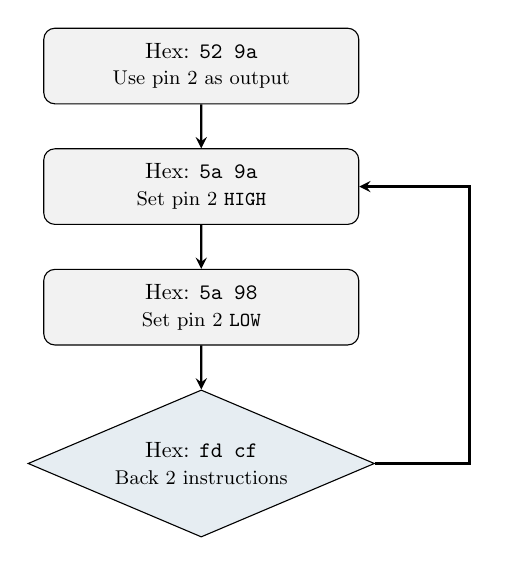
\begin{tikzpicture}[scale=0.8, every node/.style={transform shape}, node distance=0.7cm and 0.8cm]

\node (step1) [box]
    {Hex: \texttt{52 9a}\\\small Use pin 2 as output};
\node (step2) [box, below=of step1]
    {Hex: \texttt{5a 9a}\\\small Set pin 2 \texttt{HIGH}};
\node (step3) [box, below=of step2]
    {Hex: \texttt{5a 98}\\\small Set pin 2 \texttt{LOW}};
\node (step4) [jump, below=of step3]
    {Hex: \texttt{fd cf}\\\small Back 2 instructions};

\draw [arrow] (step1) -- (step2);
\draw [arrow] (step2) -- (step3);
\draw [arrow] (step3) -- (step4);

% return arrow
\draw [arrow] (step4.east) -- ++(1.5,0) node[right] {}
              |- (step2.east);

\end{tikzpicture}
\end{center}

\noindent
Writing down the hexadecimal values of the instructions one after another
gives us our first complete program in machine code:
\begin{center}
    \texttt{52 9a 5a 9a 5a 98 fd cf}
\end{center}
Each hex digit stands for exactly four bits. The complete bit patterns can be
looked up in \autoref{tab:bitmuster}. In binary notation, our program then
looks like this:
\begin{center}
    \texttt{01010010 10011010 01011010 10011010 01011010 10011000 11111101 11001111}
\end{center}

\begin{table}[ht]
    \centering
    \caption{All 4-bit numbers in decimal, hexadecimal, and binary notation}
    \label{tab:bitmuster}
    \begin{tabular}{c c c}
        \textbf{Decimal} & \textbf{Hexadecimal} & \textbf{Binary} \\
        \hline
         0 & 0  & 0000 \\
         1 & 1  & 0001 \\
         2 & 2  & 0010 \\
         3 & 3  & 0011 \\
         4 & 4  & 0100 \\
         5 & 5  & 0101 \\
         6 & 6  & 0110 \\
         7 & 7  & 0111 \\
         8 & 8  & 1000 \\
         9 & 9  & 1001 \\
        10 & A  & 1010 \\
        11 & B  & 1011 \\
        12 & C  & 1100 \\
        13 & D  & 1101 \\
        14 & E  & 1110 \\
        15 & F  & 1111 \\
    \end{tabular}
\end{table}

\noindent
The program is now completely designed. Only one last step is missing: it has
to be written into the program memory of the microprocessor – that is, into
the so-called \emph{flash} memory.

\noindent
The next section explains how to write the machine code in hexadecimal
notation into a file and transfer it to the flash memory of the
microprocessor with the program \texttt{avrdude}.

What is done today with a single command was considerably more laborious with
historical computers and microprocessors of the 1950s to 1970s:
programs were often loaded bit by bit, by flipping a toggle switch for each
individual bit (binary digit).
\footnote{Entering programs via toggle switches was perfectly normal in the
1970s – from the Altair 8800 in the hobbyist's basement to the legendary
supercomputers of Seymour Cray, the pioneer of high-performance computing.
On the Altair, you had to key in the bootloader bit by bit on the front
panel, and LEDs showed the current memory contents. Cray, too, entered the
first code by hand on his early machines before magnetic tape drives loaded
larger programs.}
Alternatively, programs were punched onto punch cards and read in
mechanically – which in principle also meant nothing more than entering many
bits in a row, just somewhat more conveniently.
Today, these old methods make a good mental model for better understanding
what the program \texttt{avrdude} actually does for us behind the scenes.

\newpage

\section[Transferring the program to the microprocessor (``flashing'' the microprocessor)]{%
    Transferring the program to the microprocessor\\
    (``flashing'' the microprocessor)%
}

\begin{figure}[ht]
\centering
\makebox[\linewidth][c]{%
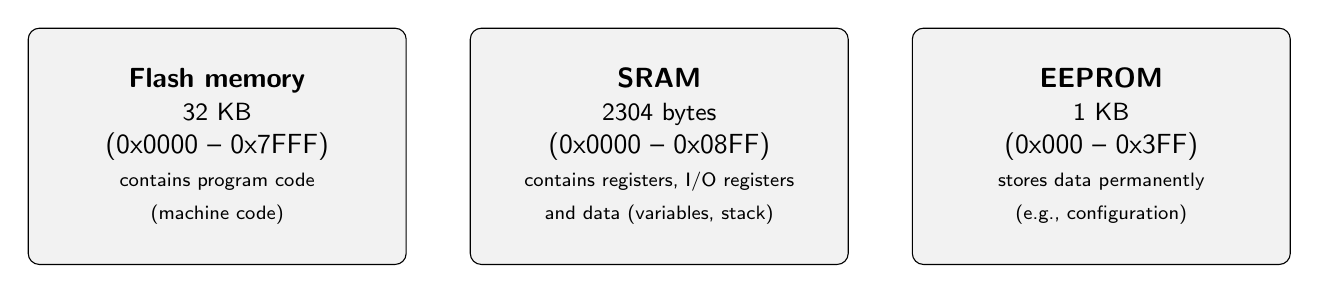
\begin{tikzpicture}[
    node distance=0.7cm and .8cm,
    font=\sffamily,
    box/.style={
        draw,
        minimum width=4.8cm,
        minimum height=3cm,
        align=center,
        rounded corners,
        fill=gray!10
    }
]

% memory blocks
\node[box] (flash) {
    \textbf{Flash memory} \\
    \small 32 KB \\
    (0x0000 – 0x7FFF) \\
    \scriptsize contains program code \\
    \scriptsize (machine code)
};

\node[box, right=of flash] (sram) {
    \textbf{SRAM} \\
    \small 2304 bytes \\
    (0x0000 – 0x08FF) \\
    \scriptsize contains registers, I/O registers \\
    \scriptsize and data (variables, stack)
};

\node[box, right=of sram] (eeprom) {
    \textbf{EEPROM} \\
    \small 1 KB \\
    (0x000 – 0x3FF) \\
    \scriptsize stores data permanently\\
    \scriptsize (e.g., configuration)
};

\end{tikzpicture}}
\caption{
    Memory organization of the ATmega328P: the flash contains the program, the
    SRAM contains registers, I/O areas, and data. The EEPROM stores
    non-volatile user data.
}
\label{fig:speicherarten}
\end{figure}

\noindent
Our microprocessor has three different kinds of memory
(\autoref{fig:speicherarten}):

\begin{itemize}
    \item
	A memory for the program – the so-called \emph{flash}. The data stored
	there are retained even when you pull the plug.
    \item
	A \emph{volatile memory} (RAM) that is available during program
	execution. The data in it are lost as soon as the power is gone.
    \item
	A so-called \emph{EEPROM} (Electrically Erasable Programmable
	Read-Only Memory), in which small amounts of data can be stored
	permanently – e.g., configurations or states that should be retained
	even after switching off.
\end{itemize}

\noindent
For now, only the flash memory matters to us – this is where our program
has to be transferred. All kinds of memory have one thing in common: they
consist of arrays of memory cells. Each cell can store exactly one byte,
i.e., 8 bits. These 8 bits can be represented compactly by two hexadecimal
digits. The memory cells are numbered consecutively – this number is called
the \emph{address}. The first address always has the value 0.
Our goal is for the program memory to look like this after flashing:


\begin{center}
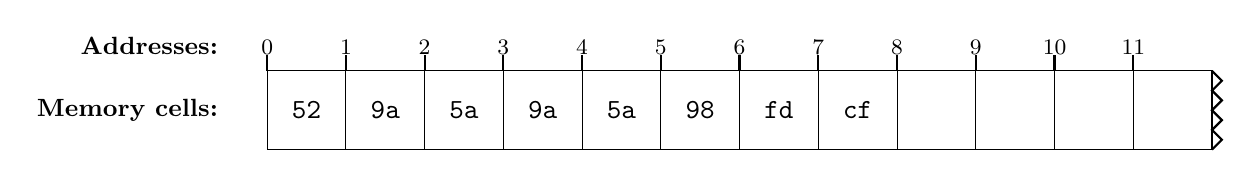
\begin{tikzpicture}
% size and spacing
\def\cellsize{1cm}

% draw 12 cells
\foreach \i in {0,...,11} {
    \draw (\i*\cellsize, 0) rectangle ++(\cellsize, \cellsize);
}

% enter the bytes into the first 8 cells
\node at (0.5*\cellsize, 0.5*\cellsize) {\ttfamily 52};
\node at (1.5*\cellsize, 0.5*\cellsize) {\ttfamily 9a};
\node at (2.5*\cellsize, 0.5*\cellsize) {\ttfamily 5a};
\node at (3.5*\cellsize, 0.5*\cellsize) {\ttfamily 9a};
\node at (4.5*\cellsize, 0.5*\cellsize) {\ttfamily 5a};
\node at (5.5*\cellsize, 0.5*\cellsize) {\ttfamily 98};
\node at (6.5*\cellsize, 0.5*\cellsize) {\ttfamily fd};
\node at (7.5*\cellsize, 0.5*\cellsize) {\ttfamily cf};

% address marks
\foreach \i in {0,...,11} {
    % small tick at the upper left corner of each cell
    \draw[thick] (\i*\cellsize, \cellsize) -- ++(0, 0.2);

    % address above the tick
    \node[anchor=south] at (\i*\cellsize, \cellsize + 2.5)
	{\footnotesize \i};
}

% labels to the left of address 0
\node[anchor=south east] at (-0.5, \cellsize + 2.5) {\small \textbf{Addresses:}};
\node[anchor=east] at (-0.5, 0.5 * \cellsize) {\small \textbf{Memory cells:}};


% jagged edge on the right
\draw[thick]
    (12*\cellsize, \cellsize) -- ++(0.125, -0.125)
    -- ++(-0.125, -0.125)
    -- ++(0.125, -0.125)
    -- ++(-0.125, -0.125)
    -- ++(0.125, -0.125)
    -- ++(-0.125, -0.125)
    -- ++(0.125, -0.125)
    -- ++(-0.125, -0.125)
    ;
\end{tikzpicture}
\end{center}

\noindent
Starting at address~0, the individual bytes should thus lie in memory one
after another. Once this has been achieved, program execution can start – it
automatically begins with the instruction stored at address~0.

After an instruction has been executed, typically the instruction located two
addresses further on in memory is executed next – because on our
microprocessor every instruction consists of exactly two bytes. Jump
instructions are an exception: they can explicitly specify that execution
continues at a different address – either forward (skipping some
instructions) or backward (jumping back).

\subsection{Intel HEX format}
A tool that transfers the machine code to the flash memory must know at least
two things about the data to be written:

\begin{enumerate}
    \item
	How many bytes have to be transferred in total.
    \item
	At which address in the flash memory the first byte should be written.
	The following bytes are then automatically stored at the subsequent
	addresses.
\end{enumerate}
This information must be provided in a suitable form – typically by means of
a special file in which the machine code and the memory addresses are
encoded. A common format for this is the so-called \emph{Intel HEX format},
which is understood by many programs – including \texttt{avrdude}.

Our machine code can be packed as follows into a file \texttt{led.hex} that
uses this format:

\vspace{15bp}
\begin{lstlisting}[
    frame=topbottom,
    caption={File \texttt{led\_pin2.hex}},
    captionpos=b
]
:08000000529A5A9A5A98FDCF5A
:00000001FF
\end{lstlisting}

\noindent
In this case, the file \texttt{led.hex} contains two so-called
\emph{records}, each shown as one line. Each record begins with a colon
(\texttt{:}) and consists of a series of hexadecimal digits that are
interpreted in groups:

\paragraph{Data line}

is a so-called \emph{data record}, which contains the actual machine code
bytes and specifies at which address in memory they should be stored.

\begin{center}
\begin{minipage}{\textwidth}
\ttfamily
\colorbox{gray!20}{\strut\textcolor{black}{:}}%
\colorbox{myblue!20}{\strut08}%
\colorbox{cyan!20}{\strut0000}%
\colorbox{violet!20}{\strut00}%
\colorbox{green!10}{\strut529A5A9A5A98FDCF}%
\colorbox{red!20}{\strut5A}

\vspace{0.2cm}

\hspace{1cm}%
\scalebox{0.74}{%
\footnotesize
\renewcommand{\arraystretch}{1.2}
\begin{tabular}{@{}l l@{}}
  \textbf{Number of data bytes:}       & \textcolor{myblue}{\texttt{08}} \\
  \textbf{Start address in memory:}    & \textcolor{cyan}{\texttt{0000}} \\
  \textbf{Record type:}                & \textcolor{violet}{\texttt{00}} (data) \\
  \textbf{Data bytes:}                 & \textcolor{green!50!black}{\texttt{52 9A 5A 9A 5A 98 FD CF}} \\
  \textbf{Checksum:}                   & \textcolor{red}{\texttt{5A}} \\
\end{tabular}
}
\end{minipage}
\end{center}

\noindent
Here once more is the meaning of the individual parts in detail:
\begin{itemize}
    \item
	\texttt{08} specifies the number of data bytes in this record
	(here: 8 bytes).
    \item
	\texttt{0000} is the start address in the flash memory at which the
	following data should be stored (in this case, address~0).
    \item
	\texttt{00} is the record type. \texttt{00} means ``normal data
	block''.
    \item
	\texttt{52 9A 5A 9A 5A 98 FD CF} are the 8 bytes of machine code that
	are to be written.
    \item
	\texttt{5A} is a checksum for error detection.
\end{itemize}

\paragraph{End-of-file line}

is a so-called \emph{end-of-file record}. It signals to the flash tool that
no further data follow. The structure is similar to that of the previous
record:

\begin{center}
\begin{minipage}{\textwidth}
\ttfamily
\colorbox{gray!20}{\strut\textcolor{black}{:}}%
\colorbox{myblue!20}{\strut00}%
\colorbox{cyan!20}{\strut0000}%
\colorbox{violet!20}{\strut01}%
\colorbox{red!20}{\strut FF}
\par\vspace{0.1cm}\null

\vspace{0.2cm}

\hspace{1cm}%
\scalebox{0.74}{%
\footnotesize
\renewcommand{\arraystretch}{1.2}
\begin{tabular}{@{}l l@{}}
  \textbf{Number of data bytes:}       & \textcolor{myblue}{\texttt{00}} \\
  \textbf{Start address in memory:}    & \textcolor{cyan}{\texttt{0000} (not relevant)} \\
  \textbf{Record type:}                & \textcolor{violet}{\texttt{01}} (end) \\
  \textbf{Data bytes:}                 & \textcolor{green!50!black}{(none)} \\
  \textbf{Checksum:}                   & \textcolor{red}{\texttt{FF}} \\
\end{tabular}
}
\end{minipage}
\end{center}

\noindent
The meaning of the individual parts in summary:

\begin{itemize}
  \item \texttt{00} — There are no data bytes in this record.
  \item \texttt{0000} — Start address (irrelevant, since no data follow).
  \item \texttt{01} — Marks this record as end-of-file.
  \item \texttt{FF} — The checksum, which here, too, serves as a check.
\end{itemize}

\noindent
This format is very compact and easy for machines to process.
Programs such as \texttt{avrdude} read this file and automatically write the
data it contains to the specified addresses in the flash memory of the
microprocessor.

\subsection{Intel HEX format: computing the checksum}

The checksum is used for error detection. For each record, the
microprocessor (or the flash tool) first receives the information on how
many data bytes it contains, followed by the actual bytes – and finally the
checksum. After reception, the checksum can be computed again and compared
with the transmitted one. If they do not match, it is clear that an error
occurred during transmission – either in the data themselves or in the
checksum.

If, on the other hand, the checksum matches the computed one, this does
\textit{not} mean that no error is guaranteed to have occurred – only that
none was detected. The checksum therefore merely reduces the probability that
a transmission error goes unnoticed.

As with all checksum methods, a compromise has to be made here:

\begin{itemize}
    \item
	If the probability of undetected errors is to be as low as possible,
	the checksum usually becomes more complex (e.g., through longer or
	cryptographic methods).
    \item
	If, on the other hand, the checksum is to be particularly simple and
	fast to compute (as in the Intel HEX format), the probability that
	certain errors go undetected increases – for example, when two faulty
	bytes happen to ``cancel each other out''.
\end{itemize}

\newpage
\noindent
The checksum in the Intel HEX format is a good compromise: very easy to
compute, but sufficiently reliable for typical flashing over stable
connections\footnote{
For high-integrity transmissions (e.g., in networks or file systems), CRCs
(cyclic redundancy checks) or cryptographic hashes are often used instead of
simple checksums.}.

\begin{tcolorbox}[
    colback=myblue!5!white,
    colframe=myblue,
    title=Computing the checksum in the Intel HEX format
]
    The Intel HEX format uses a so-called \emph{two's complement checksum}.
    Put simply: first, all bytes (except the checksum itself) are added up,
    using an 8-bit adder – that is, only the lower 8 bits of the sum are
    kept. The checksum is then exactly the number that would have to be
    added to this sum so that the result (computed with 8 bits) is
    \texttt{0} again.

    For those who like to show off with formalism: for
    $a, b \in B = \{0,\dots,2^8-1\} = \{0,\dots,255\}$,
    the 8-bit addition is defined by $a \oplus b := (a + b) \bmod 2^8$.
    For the $n$ bytes $b_1, \dots, b_n$, one then first computes
    \[
	s = b_1 \oplus b_2 \oplus \dots \oplus b_n.
    \]
    With respect to $\oplus$, the set $B$ is a finite abelian group.
    Hence, for every $s \in B$ there exists an inverse element $-s$, and
    this $-s$ is the checksum $p$ we are looking for. Thus:
    \[
	p = -s \quad \Leftrightarrow \quad p \oplus s = 0,
    \]
    so $p$ is exactly the number that has to be added to the sum $s$ to
    obtain $0$ again (modulo $2^8$).
\end{tcolorbox}

\noindent
For an example calculation by hand, you can compute directly in hexadecimal
notation. This turns an 8-digit binary calculation into a much more compact
2-digit hexadecimal calculation.

To simplify phrases such as ``the hexadecimal representation \texttt{19}'',
we will use the following convention from now on:
a prefix \texttt{0x} indicates that the digits following it are to be read
in the hexadecimal system.

So \texttt{0x19} means the number 25 in the decimal system, because:
\[
    \text{0x}19 = 1 \cdot 16 + 9 = 25.
\]
Suppose we want to compute the checksum for the three bytes
\[
    \text{0xD8} \quad \text{0xB5} \quad \text{0x19};
\]
then we proceed as follows:

\begin{enumerate}
    \item
	First, we compute the sum of the three bytes using 8-bit addition:
	\[
	    s = (\text{0xD8} \oplus \text{0xB5}) \oplus \text{0x19}
	\]
	The addition is carried out step by step. First:
	\begin{center}
	\scalebox{0.7}{%
	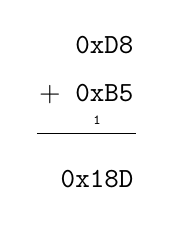
\begin{tikzpicture}[
	    font=\ttfamily, baseline=(current bounding box.south)
	]
	    \node at (0,0)     {$\phantom{+}$ 0xD8};
	    \node at (0,-0.6)  {$+$ 0xB5};
	    \node at (0,-0.9)  {$\phantom{+}$\phantom{0}\tiny\!\!\!\!\!\!1};
	    \node at (0,-1.1)  {\rule{3.4em}{0.4pt}};
	    \node at (0,-1.7)  {$\phantom{+}$0x18D};
	\end{tikzpicture}
	    }
	\end{center}
	\newpage
	Since we only compute with an 8-bit adder, we truncate the result to
	the lower 8 bits:
	\[
	    \text{0xD8} \oplus \text{0xB5}
	    = (\text{0xD8} + \text{0xB5}) \bmod 2^8
	    = \text{0x18D} \bmod 2^8 = \text{0x8D}
	\]

	Then:
	\begin{center}
	\scalebox{0.7}{%
	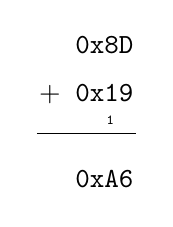
\begin{tikzpicture}[
	    font=\ttfamily, baseline=(current bounding box.south)
	]
	    \node at (0,0)     {$\phantom{+}$ 0x8D};
	    \node at (0,-0.6)  {$+$ 0x19};
	    \node at (0,-0.9)  {$\phantom{+}$\phantom{00}\tiny\!1};
	    \node at (0,-1.1)  {\rule{3.4em}{0.4pt}};
	    \node at (0,-1.7)  {$\phantom{+}$ 0xA6};
	\end{tikzpicture}
	}
	\end{center}

	Altogether, this gives $s = \text{0xA6}$.

    \item
	The checksum $p$ is obtained by subtracting $s$ from
	$2^8 = \texttt{0x100}$ and, if necessary, truncating the result to two
	digits (i.e., 8 bits). The truncation is only relevant in the special
	case $s = 0$, because then the calculation yields $p = 0x100$, but the
	correct value is of course $0x00$.

	\begin{center}
	\scalebox{0.7}{%
	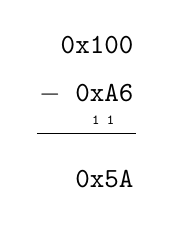
\begin{tikzpicture}[
	    font=\ttfamily, baseline=(current bounding box.south)
	]
	    \node at (0,0)     {$\phantom{-}$0x100};
	    \node at (0,-0.6)  {$-$ 0xA6};
	    \node at (0,-0.9)  {$\phantom{+}$\phantom{0}\tiny\!1 1};
	    \node at (0,-1.1)  {\rule{3.4em}{0.4pt}};
	    \node at (0,-1.7)  {$\phantom{-}$ 0x5A};
	\end{tikzpicture}
	}
	\end{center}

	This calculation of $p = (2^8 - s) \bmod 2^8$ corresponds exactly to
	the well-known method for forming the \emph{two's complement}: you
	invert the bit pattern of $s$ and then add $1$.

	For our example, this can be not only easily verified but even
	derived: we try to determine the number that has to be added to
	\texttt{0xA6} to obtain $\texttt{0x100}$.
	Along the way, we also introduce the prefix \texttt{b} to indicate a
	binary representation. We have:
	\[
	    s = \texttt{0xA6} = \texttt{b}10100110
	    \quad\Rightarrow\quad
	    \overline{s} = \texttt{b}01011001 = \texttt{0x59}
	\]
	Here, $s + \overline{s} = 2^8 - 1 = \text{0xFF}$ always holds, as can
	easily be verified in this case:
	\vspace{-0.2cm}
	\begin{center}
	\scalebox{0.7}{%
	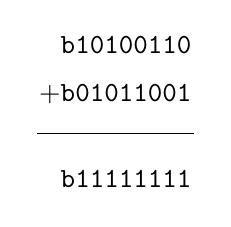
\begin{tikzpicture}[
	    font=\ttfamily, baseline=(current bounding box.south)
	]
	    \node at (0,0)     {$\phantom{+}$b10100110};
	    \node at (0,-0.6)  {$+$b01011001};
	    \node at (0,-1.1)  {\rule{5.4em}{0.4pt}};
	    \node at (0,-1.7)  {$\phantom{+}$b11111111};
	\end{tikzpicture}
	}
	\end{center}

	From this, it follows that:
	\[
	    s + \overline{s} = 2^8 - 1
	    \quad\Rightarrow\quad
	    s + (\overline{s} + 1) = 2^8
	    \quad\Rightarrow\quad
	    s \oplus (\overline{s} \oplus 1) = 0
	\]

	In other words: $\overline{s} \oplus 1$ is exactly the number that has
	to be added to $s$ in 8-bit arithmetic to obtain $0$ – and therefore
	\[
	    p = \overline{s} \oplus 1 = \texttt{0x59} \oplus 1 = \texttt{0x5A}.
	\]

\end{enumerate}


\newpage
\subsection{Flashing the microcontroller with \texttt{avrdude}}
\label{sec:avrdude}

On Linux systems, the command \texttt{ls /dev/ttyUSB*} lists the devices that
are recognized as serial interfaces – for example, a microcontroller
connected via USB. The device name found here is needed later when using
\texttt{avrdude}, in order to specify the target port correctly.
Typically, you get output like this:

\begin{lstlisting}
/dev/ttyUSB0
\end{lstlisting}

\begin{tcolorbox}[
	colback=myblue!5!white,
	colframe=myblue,
	title=Note
    ]
If several devices are connected, it can be helpful to run the command
\texttt{ls /dev/ttyUSB*} once before and once after plugging in the Arduino,
in order to identify the correct device name.
\end{tcolorbox}

\noindent
The program \texttt{avrdude} can then be used to transfer the machine program
stored in \texttt{led.hex} to the flash memory of the microcontroller. The
complete command looks roughly like this:

\begin{lstlisting}[basicstyle=\ttfamily]
avrdude -c arduino -P /dev/ttyUSB0 -p atmega328p -U flash:w:led.hex:i
\end{lstlisting}

The options stand for:

\begin{itemize}
    \item \texttt{-c arduino} \\
	Specifies which programmer is used. In this case, the Arduino
	bootloader is addressed, which can be programmed via the serial
	interface.

    \item \texttt{-P /dev/ttyUSB0} \\
	Specifies the device through which communication takes place. This is
	the name of the serial interface determined previously with
	\texttt{ls /dev/ttyUSB*}.

    \item \texttt{-p atmega328p} \\
	Specifies the target processor, here the ATmega328P (as found on an
	Arduino Uno).

    \item \texttt{-U flash:w:led.hex:i} \\
	Means: the flash memory (\texttt{flash}) is to be written
	(\texttt{w} = write) with the data from the file
	\texttt{led.hex}. The \texttt{i} at the end stands for the file
	format – here: Intel HEX.
\end{itemize}

\newpage
\section{Measuring what the program does}

As soon as the program has been written to the flash memory, the
microcontroller automatically starts executing it.

If you connect an LED to pin 2, it lights up – but with the naked eye you
cannot tell that it is blinking extremely fast. Not even a slight flicker or
a perceptible change in brightness is visible.

To check what actually happens, we use an oscilloscope in the lab.
\hyperref[fig:led-oszi1]{Figure~\ref{fig:led-oszi1}} shows the measurement of
the signal at pin 2.

\begin{figure}[ht]
    \centering
    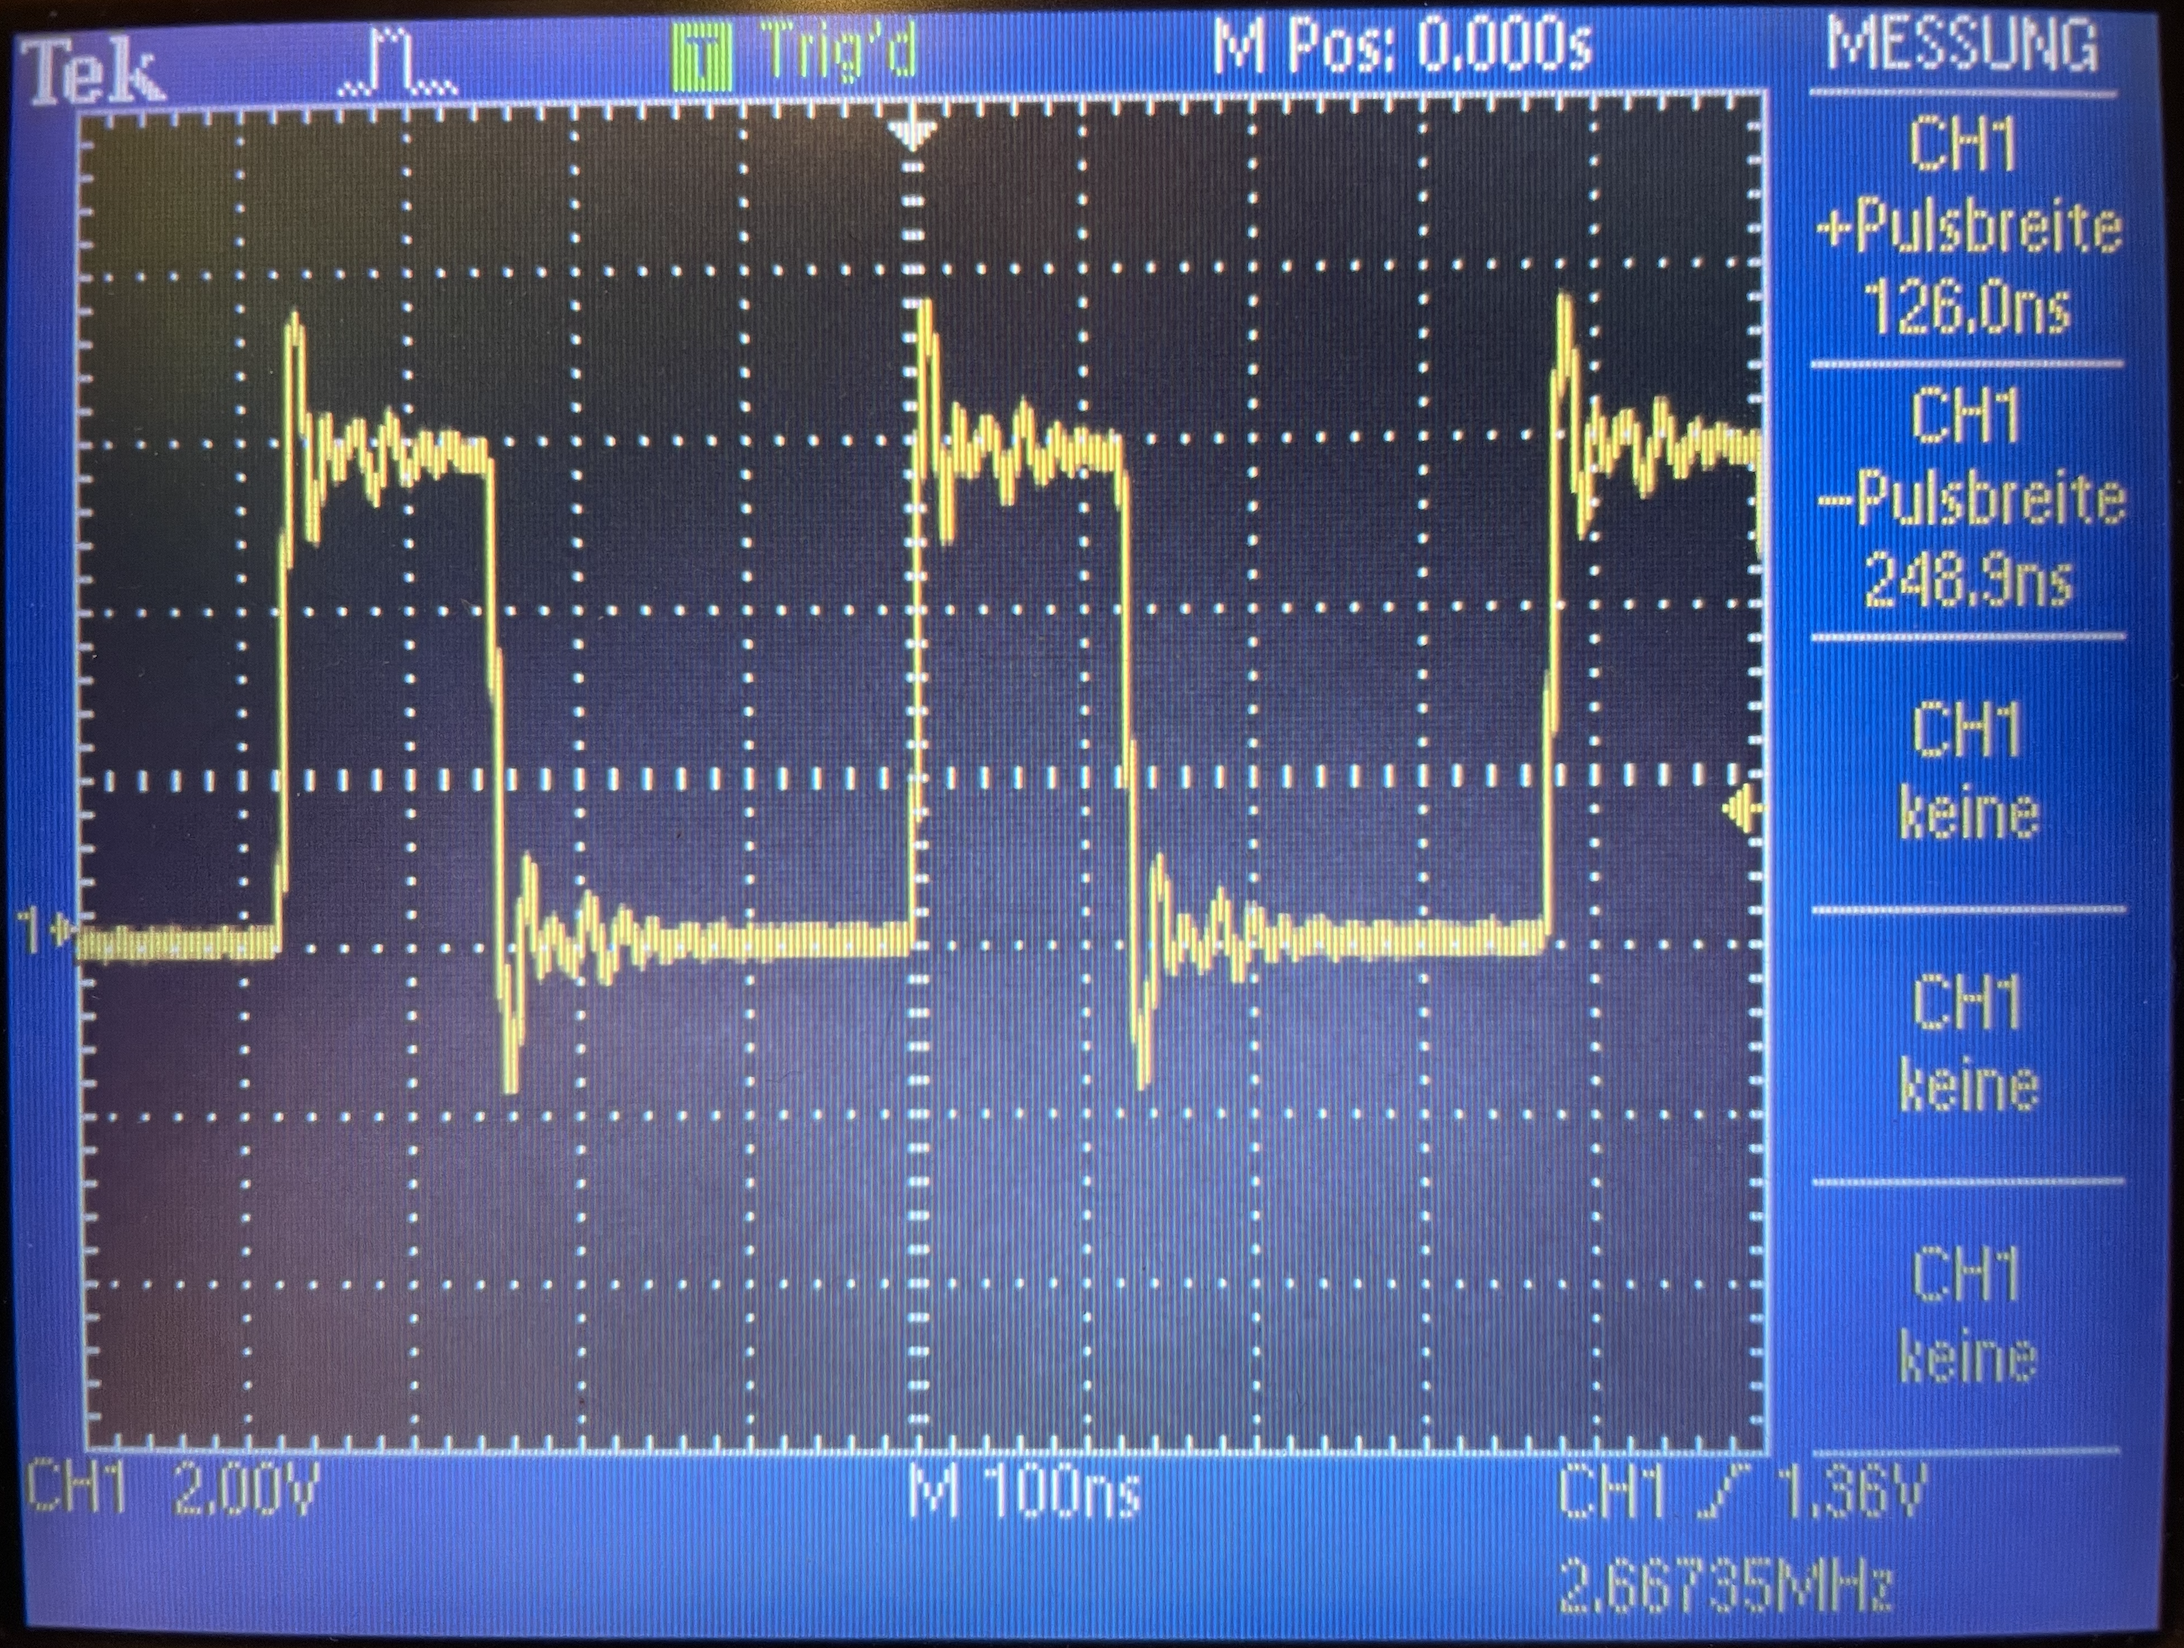
\includegraphics[width=0.8\textwidth]{led-oszi1.png}
    \caption{
	Oscilloscope measurement at pin 2 while \texttt{led.hex} is running.
	The HIGH phase lasts about 125\,ns, the LOW phase about 250\,ns – the
	signal is therefore not symmetric.
    }
    \label{fig:led-oszi1}
\end{figure}

\noindent
First, the good news: our program works as expected – the pin is alternately
set \texttt{HIGH} and \texttt{LOW}.

However, the measurement also shows that the signal is not symmetric. The
HIGH phase lasts only about 125\,ns, while the LOW phase is about twice as
long.

Why this is so is analyzed in the next section – based on the internal clock
cycles that each instruction requires.

\newpage
\section{Analyzing the program execution}

The microcontroller used in the lab (ATmega328P) runs at a clock frequency of
16\,MHz. A single CPU clock cycle therefore lasts:
\[
    \frac{1}{16\,\text{MHz}} = \frac{1}{16 \cdot 10^6}\,\text{s}
    = \frac{1000}{16} \cdot 10^{-9}\,\text{s} = 62.5\,\text{ns}.
\]
The ATmega328P datasheet specifies how many clock cycles the individual
machine instructions require. For our example, there is a pleasing
regularity: each of the instructions used takes exactly two clock cycles to
execute – including the jump instruction.
We therefore add the respective number of cycles to our flowchart:

\begin{center}
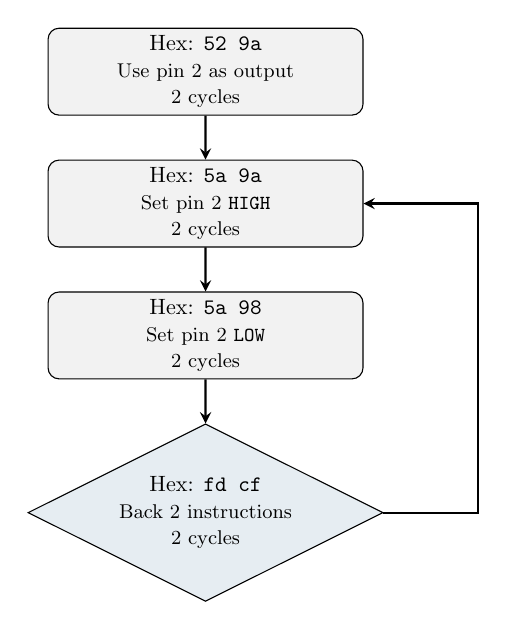
\begin{tikzpicture}[
	scale=0.8,
	every node/.style={transform shape},
	node distance=0.7cm and 0.8cm
]

\node (step1) [box]
    {Hex: \texttt{52 9a}\\\small Use pin 2 as output \\\small 2 cycles};
\node (step2) [box, below=of step1]
    {Hex: \texttt{5a 9a}\\\small Set pin 2 \texttt{HIGH}  \\\small 2 cycles};
\node (step3) [box, below=of step2]
    {Hex: \texttt{5a 98}\\\small Set pin 2 \texttt{LOW}  \\\small 2 cycles};
\node (step4) [jump, below=of step3]
    {Hex: \texttt{fd cf}\\\small Back 2 instructions  \\\small 2 cycles};

\draw [arrow] (step1) -- (step2);
\draw [arrow] (step2) -- (step3);
\draw [arrow] (step3) -- (step4);

% return arrow
\draw [arrow] (step4.east) -- ++(1.5,0) node[right] {}
              |- (step2.east);

\end{tikzpicture}
\end{center}

\noindent
\hyperref[fig:pin2-takte]{Figure~\ref{fig:pin2-takte}} shows how the state
of pin 2 changes over the course of program execution. If you keep in mind
that two CPU clock cycles correspond to 125\,ns and four cycles to 250\,ns,
this explains not only the waveform measured in
\hyperref[fig:led-oszi1]{Figure~\ref{fig:led-oszi1}}.
It also shows that, with exact knowledge of the number of cycles per
instruction, you can predict very precisely how the signal will behave –
without measuring at all.


\begin{figure}[ht]
\centering
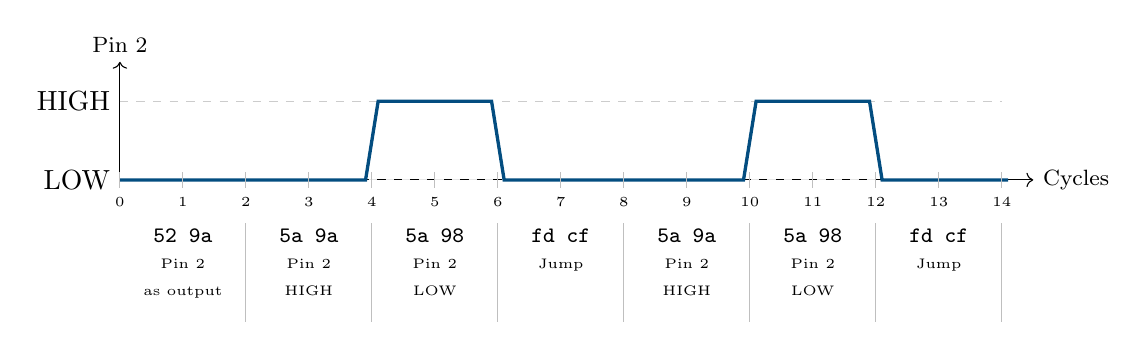
\begin{tikzpicture}[x=0.8cm, y=1cm]

% axes
\draw[->] (0,0) -- (14.5,0) node[right] {\footnotesize Cycles};
    \draw[->] (0,-0.1) -- (0,1.5) node[above] {\footnotesize Pin 2};

% y-axis labels
\draw (0,0) node[left]{LOW};
\draw (0,1) node[left]{HIGH};

% horizontal guide lines
\draw[dashed, gray!40] (0,1) -- (14,1);
\draw[dashed, gray!20] (0,0) -- (14,0);

% pin state
\draw[very thick, myblue]
    (0,0) -- (3.9,0)  % up to and including the "pin HIGH" instruction = LOW
    -- (4.1,1) -- (5.9,1)  % after the instruction: HIGH
    -- (6.1,0) -- (9.9,0) % after the LOW instruction: LOW again
    -- (10.1,1) -- (11.9,1) % HIGH
    -- (12.1,0) -- (14.1,0); % LOW

% vertical ticks at every clock cycle
\foreach \x in {0,...,14} {
    \draw[gray!50] (\x, -0.1) -- (\x, 0.1);
    \node[below] at (\x, -0.1) {\tiny \x};
}

% instruction labels below the x-axis
\newcommand{\annot}[3]{
    \node[font=\footnotesize, align=center, anchor=north] at ({(#1+#2)/2}, -0.5) {#3};
    \draw[gray!50] (#2, -0.55) -- (#2, -1.8);
}

\annot{0}{2}{\texttt{52 9a}\\\tiny Pin 2\\\tiny as output}
\annot{2}{4}{\texttt{5a 9a}\\\tiny Pin 2\\\tiny HIGH}
\annot{4}{6}{\texttt{5a 98}\\\tiny Pin 2\\\tiny LOW}
\annot{6}{8}{\texttt{fd cf}\\\tiny Jump}
\annot{8}{10}{\texttt{5a 9a}\\\tiny Pin 2\\\tiny HIGH}
\annot{10}{12}{\texttt{5a 98}\\\tiny Pin 2\\\tiny LOW}
\annot{12}{14}{\texttt{fd cf}\\\tiny Jump}

\end{tikzpicture}
\caption{
    Signal at pin 2 as a function of the CPU clock cycles. The HIGH and LOW
    states result from the machine instructions used, each of which takes
    two clock cycles.
}
\label{fig:pin2-takte}
\end{figure}

\noindent
In the next section, we will modify the program so that a symmetric signal
is produced.


\newpage

\section{Modifying the program for a symmetric signal}
\label{sec:Programmanpassung}

To produce a symmetric signal, all we have to do is make sure that pin 2
stays \texttt{HIGH} for two additional clock cycles.
Fortunately, the ATmega328P – like almost every processor – provides a
so-called \texttt{NOP} instruction (``No Operation''), which does exactly
that: nothing. According to the datasheet, this instruction takes exactly one
CPU clock cycle.

We can therefore easily modify our existing program by inserting two
\texttt{NOP} instructions directly after setting pin 2 \texttt{HIGH}. This
keeps the pin \texttt{HIGH} for a total of four clock cycles (instead of two
as before), and we get a symmetric signal with \texttt{HIGH} and
\texttt{LOW} phases of equal duration.
The new flowchart looks like this:

\begin{center}
\scalebox{0.7}{%
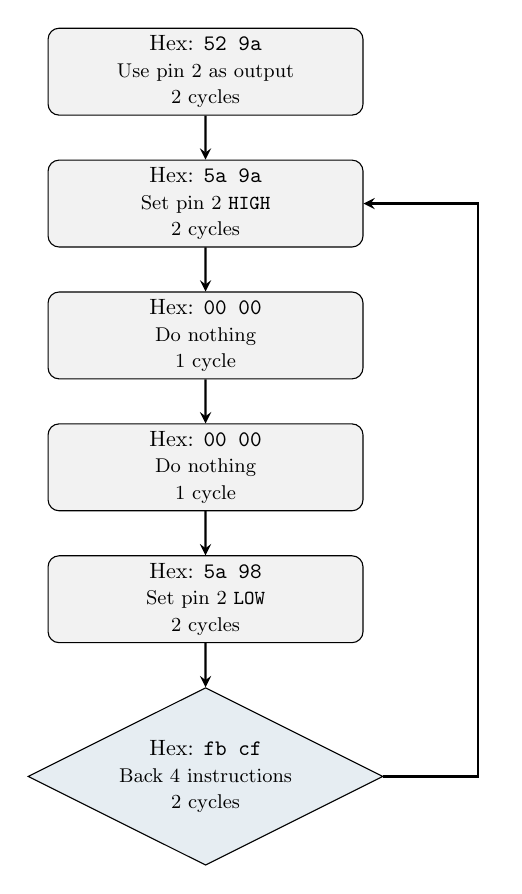
\begin{tikzpicture}[
	scale=0.8,
	every node/.style={transform shape},
	node distance=0.7cm and 0.8cm
]

\node (step1) [box]
    {Hex: \texttt{52 9a}\\\small Use pin 2 as output \\\small 2 cycles};
\node (step2) [box, below=of step1]
    {Hex: \texttt{5a 9a}\\\small Set pin 2 \texttt{HIGH}  \\\small 2 cycles};
\node (step3) [box, below=of step2]
    {Hex: \texttt{00 00}\\\small Do nothing\\\small 1 cycle};
\node (step4) [box, below=of step3]
    {Hex: \texttt{00 00}\\\small Do nothing\\\small 1 cycle};
\node (step5) [box, below=of step4]
    {Hex: \texttt{5a 98}\\\small Set pin 2 \texttt{LOW}  \\\small 2 cycles};
\node (step6) [jump, below=of step5]
    {Hex: \texttt{fb cf}\\\small Back 4 instructions  \\\small 2 cycles};

\draw [arrow] (step1) -- (step2);
\draw [arrow] (step2) -- (step3);
\draw [arrow] (step3) -- (step4);
\draw [arrow] (step4) -- (step5);
\draw [arrow] (step5) -- (step6);

% return arrow
\draw [arrow] (step6.east) -- ++(1.5,0) node[right] {}
              |- (step2.east);

\end{tikzpicture}
}
\end{center}

\noindent
Writing down the hexadecimal values of the instructions one after another,
the modified program reads:
\begin{center}
    \texttt{52 9a 5a 9a 00 00 00 00 5a 98 fb cf}
\end{center}

\noindent
Finally, the question arises of how the modified program can be converted
into the Intel HEX format. The challenge is to represent the new instructions
correctly in a hex file so that \texttt{avrdude} can write them to the flash
memory without errors.

\vspace{1em}
\vspace{16bp}
\begin{tcolorbox}[colback=myblue!5!white, colframe=myblue, title=Exercise]
    Create a valid Intel HEX file for the modified program. Pay attention to
    correct addressing and to computing the checksum correctly. Then you can
    transfer the new program to the microcontroller with \texttt{avrdude}
    and use the oscilloscope to check whether a symmetric signal is now
    produced.
\end{tcolorbox}

\medskip

\noindent
How you can quickly compute the checksum in this case in the lab under
battlefield conditions is explained in Lab Handout 1.

\section{Assembly language instead of machine code}
\label{sec:led_pin2}

We wrote the previous program for controlling the LED directly in machine
code – that is, we specified byte by byte which instructions are to be
executed. That was an instructive experience, but also a tedious one.
Fortunately, there are tools that do this work for us. A so-called
\emph{assembler} automatically translates programs written in a
human-readable symbolic language (so-called \emph{assembly code}) into
machine code. An assembly program that produces exactly the same behavior as
our modified LED program could look like this:

\begin{lstlisting}[
    frame=topbottom,
    caption={File \texttt{led\_pin2.s}},
    captionpos=b
]
        sbi     0x0a, 2     ; Configure pin 2 as output

loop:   sbi     0x0b, 2     ; Set pin 2 HIGH
        nop		    ; Do nothing
        nop		    ; Do nothing
        cbi     0x0b, 2     ; Set pin 2 LOW
	rjmp    loop        ; Back to label 'loop' (i.e., 4 instructions back)
\end{lstlisting}

\noindent
Here:
\begin{itemize}
    \item
	\texttt{sbi} stands for ``Set Bit'' – a specific bit in an I/O
	register is set to \texttt{1}.
    \item
	\texttt{cbi} stands for ``Clear Bit'' – a specific bit is set to
	\texttt{0}.
    \item
	\texttt{nop} is a so-called no-operation – the instruction does
	nothing but takes up one CPU clock cycle.
    \item
	\texttt{rjmp} is a relative jump instruction – it jumps back by a
	certain number of instructions (here: to the label \texttt{loop}).
\end{itemize}

\noindent
The advantage: the code is much more readable than a sequence of bytes such
as \texttt{52 9a ...}. You can see immediately what is meant – and the risk
of errors is much lower.

\subsection{From assembly code to an Intel HEX file}

An assembly program like the one shown above can be translated into machine
code with the tool \texttt{avr-as}. In the good old days, that was often all
there was to it: the generated machine code could be executed directly or
saved as an Intel HEX file – done. The world was simple, and so were the
tools.

Today, systems are more complex – and so are the toolchains. To deal with
this complexity, the tasks are divided into smaller steps:

\begin{itemize}
    \item
	\texttt{avr-as} first generates a so-called \emph{object file}
	(\texttt{.o}) with machine code, but still without complete address
	information.

    \item
	This file is further processed by the \emph{linker} \texttt{avr-ld}.
        The linker replaces symbolic jump targets – such as the label
        \texttt{loop} in our assembly program – with concrete addresses.
        This produces an executable file in the so-called
        \emph{ELF format} (Executable and Linkable Format), a modern
        standard on Linux.

    \item
	Since the ATmega328P of course does not understand the ELF format
	(after all, it comes from the good old days and, as is only proper,
	expects raw machine code), the machine code has to be extracted from
	the ELF file with \texttt{avr-objcopy} and converted into the
	\emph{Intel HEX format} – a format suitable for flashing the
	microcontroller.

\end{itemize}

\noindent The complete toolchain thus looks like this:

\begin{lstlisting}
avr-as -o led_pin2.o led_pin2.s
avr-ld -mavr5 -o led_pin2.elf led_pin2.o
avr-objcopy -O ihex -R .eeprom led_pin2.elf led_pin2.hex
\end{lstlisting}

\noindent
Before flashing the microcontroller, you can look at the contents of the file
\texttt{led\_pin2.hex} – it should match exactly the Intel HEX file created
by hand in \autoref{sec:Programmanpassung}. The microcontroller can then be
flashed with \texttt{avrdude}, as already shown in \autoref{sec:avrdude}.

\vspace{15bp}
\subsection{A Makefile for Linux and macOS}


\begin{listing}[htbp]
\centering
\caption{
    File \texttt{Makefile} for translating assembly programs on Linux and
    macOS. This version processes \texttt{.s} files only.
}
\label{lst:Makefile_asm}
\vspace{1em}
\begin{minipage}{0.95\textwidth}
\begin{lstlisting}[
    language=make,
    numbers=left,
    numberstyle=\scriptsize,
    stepnumber=1,
    numbersep=4pt,
    basicstyle=\ttfamily\small
]
# This version only processes assembly programs (*.s)
# Later, an extended Makefile will also support C.

SOURCES := $(wildcard *.s)
OBJECTS := $(SOURCES:.s=.o)
ELFS    := $(SOURCES:.s=.elf)
HEXS    := $(SOURCES:.s=.hex)

all: $(HEXS)

%.o: %.s
        avr-as -o $@ $<

%.elf: %.o
        avr-ld -mavr5 -o $@ $<

%.hex: %.elf
        avr-objcopy -O ihex -R .eeprom $< $@

clean:
        $(RM) $(OBJECTS) $(ELFS) $(HEXS)

ifeq ($(MAKECMDGOALS),upload)
ifeq ($(shell uname), Linux)
PORT := $(shell ls /dev/ttyUSB* 2>/dev/null | head -n 1)
else
PORT := $(shell ls /dev/cu.usb* 2>/dev/null | head -n 1)
endif # uname
endif # MAKECMDGOALS == upload

upload: $(HEX)
        @if [ -z "$(HEX)" ]; then \
            echo "Usage: make upload HEX=<filename.hex>"; \
            false; \
        fi
        @if [ -z "$(PORT)" ]; then \
            echo "no USB device found"; \
            false; \
        fi
        avrdude -c arduino -P $(PORT) -p atmega328p -U flash:w:$(HEX):i
\end{lstlisting}
\end{minipage}
\end{listing}

\noindent
To make working with several assembly files easier, we use the
\texttt{Makefile} shown in \autoref{lst:Makefile_asm}. It ensures that a
matching Intel HEX file is automatically generated for every \texttt{.s}
file. For this, the Makefile should be located in the same directory as the
assembly files. To translate, all you need is the command:

\begin{lstlisting}
make
\end{lstlisting}
In addition, with
\begin{lstlisting}
make upload HEX=led_pin2.hex
\end{lstlisting}
you can transfer a specific hex file – such as \texttt{led\_pin2.hex} here –
to the microcontroller. In principle, the ``Verify'' button in the Arduino
IDE hides a call to \texttt{make}, and the ``Upload'' button a call to
\texttt{make upload HEX=\dots}.

\medskip
For the translation, the toolchain described above, consisting of
\texttt{avr-as}, \texttt{avr-ld}, \texttt{avr-objcopy}, and \texttt{avrdude},
is used – but in a sensible combination. More precisely:

\begin{itemize}
\item
    \texttt{avr-as} generates \texttt{led\_pin2.o} only if
    \texttt{led\_pin2.s} has changed – that is, if the source file is newer
    than the object file or the latter does not exist yet.
\item
    \texttt{avr-ld} generates a new \texttt{led\_pin2.elf} only if
    \texttt{led\_pin2.o} has changed.
\item
    \texttt{avr-objcopy} generates a new \texttt{led\_pin2.hex} only if
    \texttt{led\_pin2.elf} has changed.
\end{itemize}

\noindent
This saves unnecessary work – and that is precisely the strength of
\texttt{make}.
\medskip
If, on the other hand, a file is uploaded directly with
\begin{lstlisting}
make upload HEX=led_pin2.hex
\end{lstlisting}
\newpage
\noindent
then \texttt{make} automatically checks whether the specified file is up to
date – that is, whether steps such as translating from \texttt{.s} to
\texttt{.o}, linking to the \texttt{.elf} file, or generating the
\texttt{.hex} file might be required first. These dependencies, too, are
reliably detected and executed in the correct order – without any further
action on your part.

Even if you would not suspect it at first glance: what you see in the
\texttt{Makefile} is actually a programming language. Its syntax and
user-friendliness are certainly debatable – but it is functional, no doubt:
it automatically detects dependencies between files, decides which
intermediate steps are necessary, and executes them in the correct order.

However, some things hurt to look at – for example, the block in
lines~23--29. The fact that the \texttt{ifeq} constructs there are not
indented is not an oversight but, unfortunately, necessary obedience:
\texttt{make} accepts directives such as \texttt{ifeq}, \texttt{endif},
\texttt{define}, etc.\ only at the beginning of a line – just like simple
assignments such as \texttt{PORT~:=~...}. Visual indentation for better
readability is simply not allowed. Especially if you – like the author – are
allergic to inconsistent indentation in~C and consider it a blessing that
Python enforces indentation, the syntax of \texttt{make} sometimes feels
like a little journey back in time to the 1980s.


The Makefile in \autoref{lst:Makefile_asm} will be provided to you in the
lab. How to extend it so that C programs can be processed as well will be
part of a lab task later on.
It is not necessary to know every detail about Makefiles for this. To begin
with, it is enough if you understand how the dependencies described above
are implemented in the Makefile.

Line~11, for example, contains the rule for how to generate a \texttt{.o}
file from a \texttt{.s} file – provided that an update is necessary
(i.e., the \texttt{.o} file is missing or older than the corresponding
\texttt{.s} file).
Line~12 contains the corresponding command,
\texttt{avr-as -o \$@ \$<},
where \texttt{\$@} is automatically replaced by the name of the target file
(i.e., the \texttt{.o} file) and \texttt{\$<} by the name of the source file
(i.e., the \texttt{.s} file).


Altogether, the Makefile thus describes a directed graph of dependencies, as
visualized in \autoref{fig:makegraph}: each step builds on the previous one,
and \texttt{make} ensures that all necessary commands are executed in the
correct order – but only when they are really required.


\vspace{57bp}
\begin{figure}[ht]
\centering
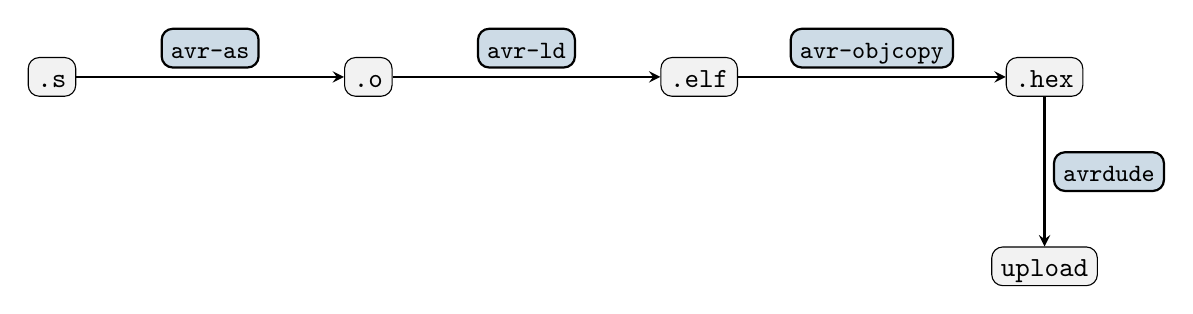
\begin{tikzpicture}[
  node distance=1.4cm and 3.4cm,
  every node/.style={draw, rounded corners, fill=gray!10, font=\ttfamily},
  arrow/.style={->, thick, >=stealth},
  text height=1.7ex,
  text depth=0pt,
  minimum height=1.8ex,
  align=center
]

\node (s)   {.s};
\node (o)   [right=of s] {.o};
\node (elf) [right=of o] {.elf};
\node (hex) [right=of elf] {.hex};
\node (upload) [below=of hex, yshift=-0.5cm] {upload};

\draw[arrow] (s)   -- (o)     node[midway, above=3pt, fill=myblue!20]  {\small avr-as};
\draw[arrow] (o)   -- (elf)   node[midway, above=3pt, fill=myblue!20]  {\small avr-ld};
\draw[arrow] (elf) -- (hex)   node[midway, above=3pt, fill=myblue!20]  {\small avr-objcopy};
\draw[arrow] (hex) -- (upload) node[midway, right=3pt, fill=myblue!20] {\small avrdude};

\end{tikzpicture}
\caption{
    Dependency graph for generating a \texttt{.hex} file and the subsequent
    upload. The tools \texttt{avr-as}, \texttt{avr-ld}, and
    \texttt{avr-objcopy} generate the \texttt{.hex} file, which is finally
    transferred to the microcontroller by \texttt{avrdude}.
}
\label{fig:makegraph}
\end{figure}


\newpage
\subsection{Blinking more elegantly with exclusive OR}

The following program – like the previous one – makes an LED blink so that it
is alternately on for 250\,ns and off for 250\,ns. So once again, a clean,
symmetric signal is produced.

The difference lies in the code: this time, registers are used – and, above
all, a new instruction, namely an exclusive OR. This logical operation is
often abbreviated as \textbf{XOR} (for \emph{exclusive OR}).
On the ATmega328P, however, the corresponding machine instruction is called
\textbf{EOR} – as in line~5 of the following program.

Let us first take a look at the code before we work out in detail how it
works and what role registers and other special features play:

\begin{lstlisting}[
    frame=topbottom,
    numbers=left,
    numberstyle=\scriptsize,
    caption={File \texttt{led\_pin2\_xor.s}},
    captionpos=b,
    label={lst:led_pin2_xor}
]
	ldi	r19,	4	    ; r19 = mask for pin 2 (note: 4 = 2^2)
	out	0x0a,	r19	    ; pin 2 as output
	ldi	r18,	0	    ; r18 = 0
loop:
	eor	r18,	r19	    ; r18 = r18 XOR r19 ("toggle")
	out	0x0b,	r18	    ; set pin 2 HIGH or LOW
	rjmp	loop
\end{lstlisting}


\medskip
\noindent
Before we analyze the new code step by step, let us first clarify some
important terms and concepts:

\begin{itemize}
    \item
	What are registers – and how do they differ from normal memory
	cells?
    \item
	What exactly are I/O registers – and how can they be used to control
	the pins of the microcontroller?
    \item
	How can a pin be configured as an input or output?
    \item
	And how can it be set specifically \texttt{HIGH} or \texttt{LOW}?
\end{itemize}
\noindent
The following sections answer all of these questions. They not only help you
understand the new code better but, in retrospect, also explain many details
of our very first assembly program (\autoref{sec:led_pin2}).

By the way, in the lab you are welcome to simply try out first whether this
new program really produces a 250\,ns–250\,ns blink signal again – just like
the previous one. If the oscilloscope shows a familiar pattern, that is
already a good sign. And now let us look in detail at how exactly this
program works.

\paragraph{Registers: computing only with registers}

Registers are special memory cells that the processor can use directly for
arithmetic operations. The ATmega328P has 32 of them – each 8~bits wide –
named \texttt{r0}, \texttt{r1}, \texttt{r2}, \dots, \texttt{r31}.
Technically, on the ATmega328P the registers are located in the same data
space as the SRAM (\autoref{fig:speicherarten}), which is also used for
local and global variables – \textit{the exact structure of this memory area
is shown in} \autoref{fig:sram-struktur}.

\begin{figure}[htbp]
\centering
\begin{center}
\scalebox{0.85}{%
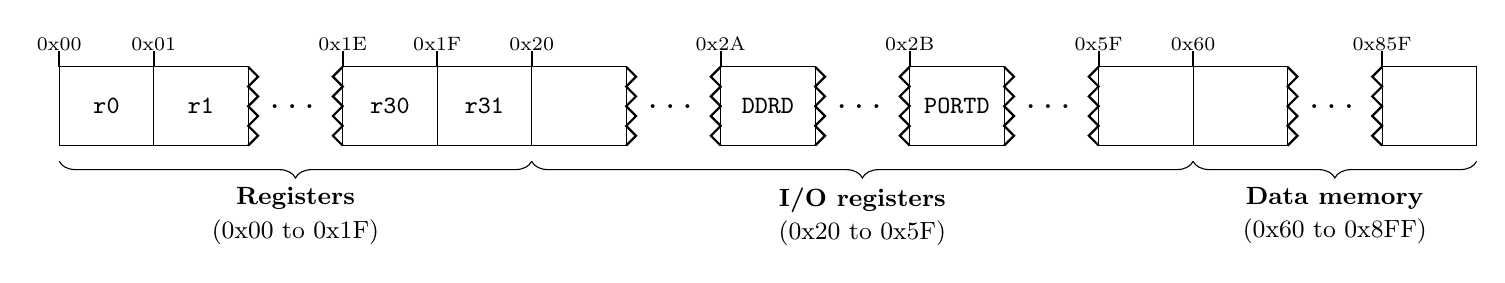
\begin{tikzpicture}
\def\cellsizex{1.2cm}
\def\cellsizey{1cm}

% r0
\draw (0, 0) rectangle ++(\cellsizex, \cellsizey);
\node at (0.5*\cellsizex, 0.5*\cellsizey) {\ttfamily\small r0};
\draw[thick] (0, \cellsizey) -- ++(0, 0.2);
\node[anchor=south] at (0, \cellsizey + 2.5) {\scriptsize 0x00};

% r1
\draw (1*\cellsizex, 0) rectangle ++(\cellsizex, \cellsizey);
\node at (1.5*\cellsizex, 0.5*\cellsizey) {\ttfamily\small r1};
\draw[thick] (1*\cellsizex, \cellsizey) -- ++(0, 0.2);
\node[anchor=south] at (1*\cellsizex, \cellsizey + 2.5) {\scriptsize 0x01};

% zigzag left
\draw[thick]
    (2*\cellsizex, \cellsizey) -- ++(0.125, -0.125)
    -- ++(-0.125, -0.125)
    -- ++(0.125, -0.125)
    -- ++(-0.125, -0.125)
    -- ++(0.125, -0.125)
    -- ++(-0.125, -0.125)
    -- ++(0.125, -0.125)
    -- ++(-0.125, -0.125)
    ;

\node at (2.5*\cellsizex, 0.5*\cellsizey) {\Large\textellipsis};

% zigzag right (left of r30)
\draw[thick]
    (3*\cellsizex, \cellsizey) -- ++(-0.125, -0.125)
    -- ++(0.125, -0.125)
    -- ++(-0.125, -0.125)
    -- ++(0.125, -0.125)
    -- ++(-0.125, -0.125)
    -- ++(0.125, -0.125)
    -- ++(-0.125, -0.125)
    -- ++(0.125, -0.125)
    ;

% r30
\draw (3*\cellsizex, 0) rectangle ++(\cellsizex, \cellsizey);
\node at (3.5*\cellsizex, 0.5*\cellsizey) {\ttfamily\small r30};
\draw[thick] (3*\cellsizex, \cellsizey) -- ++(0, 0.2);
\node[anchor=south] at (3*\cellsizex, \cellsizey + 2.5) {\scriptsize 0x1E};

% r31
\draw (4*\cellsizex, 0) rectangle ++(\cellsizex, \cellsizey);
\node at (4.5*\cellsizex, 0.5*\cellsizey) {\ttfamily\small r31};
\draw[thick] (4*\cellsizex, \cellsizey) -- ++(0, 0.2);
\node[anchor=south] at (4*\cellsizex, \cellsizey + 2.5) {\scriptsize 0x1F};


% brace with label
\draw [decorate, decoration={brace, mirror, amplitude=6pt}]
      (0*\cellsizex, -0.2) -- (5*\cellsizex, -0.2)
      node[midway, below=6pt, align=center] {\small\textbf{Registers}\\\small(0x00 to 0x1F)};

\draw (5*\cellsizex, 0) rectangle ++(\cellsizex, \cellsizey);
\draw[thick] (5*\cellsizex, \cellsizey) -- ++(0, 0.2);
\node[anchor=south] at (5*\cellsizex, \cellsizey + 2.5) {\scriptsize 0x20};

% zigzag left
\draw[thick]
    (6*\cellsizex, \cellsizey) -- ++(0.125, -0.125)
    -- ++(-0.125, -0.125)
    -- ++(0.125, -0.125)
    -- ++(-0.125, -0.125)
    -- ++(0.125, -0.125)
    -- ++(-0.125, -0.125)
    -- ++(0.125, -0.125)
    -- ++(-0.125, -0.125)
    ;

\node at (6.5*\cellsizex, 0.5*\cellsizey) {\Large\textellipsis};

\draw[thick]
    (7*\cellsizex, \cellsizey) -- ++(-0.125, -0.125)
    -- ++(0.125, -0.125)
    -- ++(-0.125, -0.125)
    -- ++(0.125, -0.125)
    -- ++(-0.125, -0.125)
    -- ++(0.125, -0.125)
    -- ++(-0.125, -0.125)
    -- ++(0.125, -0.125)
    ;
\draw (7*\cellsizex, 0) rectangle ++(\cellsizex, \cellsizey);
\draw[thick] (7*\cellsizex, \cellsizey) -- ++(0, 0.2);
\node at (7.5*\cellsizex, 0.5*\cellsizey) {\ttfamily\small DDRD};
\node[anchor=south] at (7*\cellsizex, \cellsizey + 2.5) {\scriptsize 0x2A};

% zigzag left
\draw[thick]
    (8*\cellsizex, \cellsizey) -- ++(0.125, -0.125)
    -- ++(-0.125, -0.125)
    -- ++(0.125, -0.125)
    -- ++(-0.125, -0.125)
    -- ++(0.125, -0.125)
    -- ++(-0.125, -0.125)
    -- ++(0.125, -0.125)
    -- ++(-0.125, -0.125)
    ;

\node at (8.5*\cellsizex, 0.5*\cellsizey) {\Large\textellipsis};

\draw[thick]
    (9*\cellsizex, \cellsizey) -- ++(-0.125, -0.125)
    -- ++(0.125, -0.125)
    -- ++(-0.125, -0.125)
    -- ++(0.125, -0.125)
    -- ++(-0.125, -0.125)
    -- ++(0.125, -0.125)
    -- ++(-0.125, -0.125)
    -- ++(0.125, -0.125)
    ;
\draw (9*\cellsizex, 0) rectangle ++(\cellsizex, \cellsizey);
\draw[thick] (9*\cellsizex, \cellsizey) -- ++(0, 0.2);
\node at (9.5*\cellsizex, 0.5*\cellsizey) {\ttfamily\small PORTD};
\node[anchor=south] at (9*\cellsizex, \cellsizey + 2.5) {\scriptsize 0x2B};
% zigzag left
\draw[thick]
    (10*\cellsizex, \cellsizey) -- ++(0.125, -0.125)
    -- ++(-0.125, -0.125)
    -- ++(0.125, -0.125)
    -- ++(-0.125, -0.125)
    -- ++(0.125, -0.125)
    -- ++(-0.125, -0.125)
    -- ++(0.125, -0.125)
    -- ++(-0.125, -0.125)
    ;

\node at (10.5*\cellsizex, 0.5*\cellsizey) {\Large\textellipsis};

\draw[thick]
    (11*\cellsizex, \cellsizey) -- ++(-0.125, -0.125)
    -- ++(0.125, -0.125)
    -- ++(-0.125, -0.125)
    -- ++(0.125, -0.125)
    -- ++(-0.125, -0.125)
    -- ++(0.125, -0.125)
    -- ++(-0.125, -0.125)
    -- ++(0.125, -0.125)
    ;
\draw (11*\cellsizex, 0) rectangle ++(\cellsizex, \cellsizey);
\draw[thick] (11*\cellsizex, \cellsizey) -- ++(0, 0.2);
\node[anchor=south] at (11*\cellsizex, \cellsizey + 2.5) {\scriptsize 0x5F};
% brace with label
\draw [decorate, decoration={brace, mirror, amplitude=6pt}]
      (5*\cellsizex, -0.2) -- (12*\cellsizex, -0.2)
      node[midway, below=6pt, align=center] {\small\textbf{I/O registers}\\\small(0x20 to 0x5F)};


\draw (12*\cellsizex, 0) rectangle ++(\cellsizex, \cellsizey);
\draw[thick] (12*\cellsizex, \cellsizey) -- ++(0, 0.2);
\node[anchor=south] at (12*\cellsizex, \cellsizey + 2.5) {\scriptsize 0x60};
% zigzag left
\draw[thick]
    (13*\cellsizex, \cellsizey) -- ++(0.125, -0.125)
    -- ++(-0.125, -0.125)
    -- ++(0.125, -0.125)
    -- ++(-0.125, -0.125)
    -- ++(0.125, -0.125)
    -- ++(-0.125, -0.125)
    -- ++(0.125, -0.125)
    -- ++(-0.125, -0.125)
    ;

\node at (13.5*\cellsizex, 0.5*\cellsizey) {\Large\textellipsis};

% zigzag right (left of r30)
\draw[thick]
    (14*\cellsizex, \cellsizey) -- ++(-0.125, -0.125)
    -- ++(0.125, -0.125)
    -- ++(-0.125, -0.125)
    -- ++(0.125, -0.125)
    -- ++(-0.125, -0.125)
    -- ++(0.125, -0.125)
    -- ++(-0.125, -0.125)
    -- ++(0.125, -0.125)
    ;
\draw (14*\cellsizex, 0) rectangle ++(\cellsizex, \cellsizey);
\draw[thick] (14*\cellsizex, \cellsizey) -- ++(0, 0.2);
\node[anchor=south] at (14*\cellsizex, \cellsizey + 2.5) {\scriptsize 0x85F};

% brace with label
\draw [decorate, decoration={brace, mirror, amplitude=6pt}]
      (12*\cellsizex, -0.2) -- (15*\cellsizex, -0.2)
      node[midway, below=6pt, align=center] {\small\textbf{Data memory}\\\small(0x60 to 0x8FF)};


\end{tikzpicture}
} % scalebox
\end{center}
\caption{
    Schematic representation (not to scale) of the SRAM area of the
    ATmega328P. Shown are the memory cells for the registers as well as the
    memory addresses with which the direction of the pins can be set
    (e.g., DDRD) or the outputs can be set directly (e.g., PORTD).
}
\label{fig:sram-struktur}
\end{figure}

The special thing is: arithmetic operations such as addition, comparison, or
logical operations can be performed exclusively with registers. If you want
to work with variables located in normal SRAM, you first have to load them
into a register – and, if necessary, write them back after the computation.

\noindent
To be able to compute with registers at all, they first have to be assigned
a value. A simple way to do this is the instruction \texttt{ldi}, which
stands for ``load immediate'', i.e., ``load directly''. It lets you write a
constant directly into a register:

\begin{lstlisting}
    ldi     r19, 4     ; r19 gets the value 4
    ldi     r18, 0     ; r18 gets the value 0
\end{lstlisting}

\noindent
In this example, register \texttt{r19} is preloaded with the value
\texttt{4} – i.e., with a bit mask in which only bit 2 is set. Register
\texttt{r18} gets the value \texttt{0}.

Now a typical arithmetic operation comes into play: the so-called
\emph{exclusive OR} operation (XOR), which is implemented in the ATmega328P
assembly language by the instruction \texttt{eor}. It works bitwise and
yields a \texttt{1} only if the two operands have different bits at the
respective position. The instruction

\begin{lstlisting}
    eor     r18, r19
\end{lstlisting}

\noindent
causes the contents of \texttt{r18} to be replaced by \texttt{r18 XOR r19}.
Since \texttt{r18} previously had the value \texttt{0}, and \texttt{r19} has
the value \texttt{4}, the result is \texttt{r18 = 0 XOR 4 = 4}.
If the instruction

\begin{lstlisting}
    eor     r18, r19
\end{lstlisting}

\noindent
is then executed again, \texttt{r18 = 4 XOR 4 = 0}. The original value has
thus been cleared again. Repeated application of this instruction therefore
toggles the contents of \texttt{r18} between \texttt{0} and \texttt{4} –
exactly this behavior is what we use to set the pin state alternately
\texttt{HIGH} and \texttt{LOW}:

\begin{center}
\begin{minipage}{0.42\textwidth}
\makebox[\linewidth][l]{%
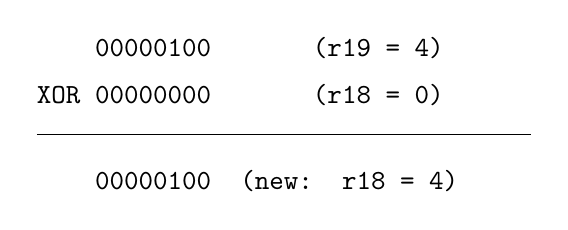
\begin{tikzpicture}[font=\ttfamily]
\node[anchor=west]  at (0,0)     {\phantom{XOR }00000100 \ \ \ \ \ \ (r19 = 4)};
\node[anchor=west]  at (0,-0.6)  {XOR 00000000 \ \ \ \ \ \  (r18 = 0)};
\node[anchor=west]  at (0,-1.1)  {\rule{17em}{0.4pt}};
\node[anchor=west]  at (0,-1.7)  {\phantom{XOR }00000100 \ (new: r18 = 4)};
\end{tikzpicture}}
\end{minipage}
\hfill
\begin{minipage}{0.42\textwidth}
\makebox[\linewidth][l]{%
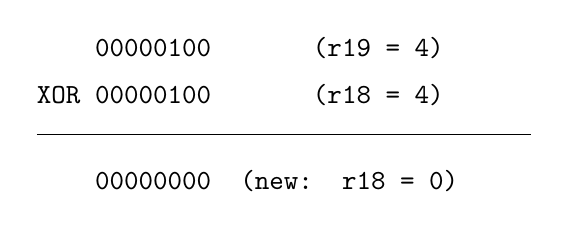
\begin{tikzpicture}[font=\ttfamily]
\node[anchor=west]  at (0,0)     {\phantom{XOR }00000100 \ \ \ \ \ \ (r19 = 4)};
\node[anchor=west]  at (0,-0.6)  {XOR 00000100 \ \ \ \ \ \  (r18 = 4)};
\node[anchor=west]  at (0,-1.1)  {\rule{17em}{0.4pt}};
\node[anchor=west]  at (0,-1.7)  {\phantom{XOR }00000000 \ (new: r18 = 0)};
\end{tikzpicture}}
\end{minipage}
\end{center}

\paragraph{I/O registers: the interface to the pins}

I/O registers (input/output registers) are special memory cells in the SRAM
area through which the pins of the microcontroller can be controlled. For
pins~0–7 of our microprocessor, the addresses \texttt{0x2A} and
\texttt{0x2B} are particularly relevant:

\begin{itemize}
    \item
	\texttt{0x2A} corresponds to the so-called \texttt{DDRD} register. If
	the bit with index~2 is set there, pin~2 is configured as an output.
\newpage
    \item
	\texttt{0x2B} corresponds to the \texttt{PORTD} register. If the bit
	with index~2 is set there, pin~2 is at a HIGH level – otherwise it is
	LOW.
\end{itemize}

\noindent
Interestingly, we already used these registers in our first assembly program
(see \autoref{sec:led_pin2}) – but with different addresses. There we had,
for example:

\begin{lstlisting}
    sbi     0x0a, 2    ; Configure pin 2 as output
    sbi     0x0b, 2    ; Set pin 2 HIGH
    cbi     0x0b, 2    ; Set pin 2 LOW
\end{lstlisting}

\noindent
Here, the address \texttt{0x0a} was used instead of \texttt{0x2A}, and
\texttt{0x0b} instead of \texttt{0x2B}.

\noindent
The reason: the instructions \texttt{sbi} (set bit) and \texttt{cbi} (clear
bit) are specifically intended for accessing I/O registers directly. They
operate only on addresses in the range \texttt{0x00} to \texttt{0x1F}, which
corresponds to the first 32~I/O registers. Internally, an offset of
\texttt{0x20} is automatically added when these instructions are executed.
This saves valuable bits in the machine instruction, since only a small
address range has to be encoded.



\paragraph{Overwriting an I/O register completely}

In the previous example, individual bits in the I/O registers were
specifically set or cleared – e.g., using the instructions \texttt{sbi} (set
bit) or \texttt{cbi} (clear bit). An alternative is to overwrite the entire
register at once. This is not only more compact and clearer but also more
efficient: while \texttt{sbi} and \texttt{cbi} each take two CPU clock
cycles, a complete write access with the instruction \texttt{out} takes only
a single cycle.

\medskip
\noindent
As a reminder:
\begin{itemize}
    \item
	The register \texttt{DDRD} (address \texttt{0x2A}) determines which
	pins are used as outputs. To enable only pin~2 as an output, you write
	the number \texttt{4} (= $2^2$) into the \texttt{DDRD} register – that
	is, exactly the bit with index~2.
    \item
	The register \texttt{PORTD} (address \texttt{0x2B}) determines whether
	an output pin is \texttt{HIGH} or \texttt{LOW}. To set pin~2
	\texttt{HIGH}, you likewise write the value \texttt{4} into it. To set
	it \texttt{LOW}, the value \texttt{0} is sufficient.
\end{itemize}

\medskip
\noindent
For this, you use the instruction \texttt{out}, which requires two
operands:
\begin{itemize}
    \item
	the target address – e.g., \texttt{0x2A} for \texttt{DDRD} or
	\texttt{0x2B} for \texttt{PORTD}
    \item
	a register that contains the value to be written
\end{itemize}
This is exactly what the following example does:
\begin{lstlisting}
    ldi     r19, 4        ; set bit 2
    out     0x0A, r19     ; configure pin 2 as output (DDRD)
    out     0x0B, r19     ; set pin 2 HIGH (PORTD)
\end{lstlisting}


\noindent
Important: with \texttt{out}, too – as with \texttt{sbi} and \texttt{cbi} –
an offset of \texttt{0x20} is added internally to the specified address. In
the example above, the writes therefore actually go to address \texttt{0x2A}
and address \texttt{0x2B}, respectively, which are exactly the physical
memory addresses of \texttt{DDRD} and \texttt{PORTD} (see
\autoref{fig:sram-struktur}).

\medskip
\noindent
We have now understood every instruction in \autoref{lst:led_pin2_xor}.
If we now also analyze the program flow, it becomes clear why the signal at
pin 2 is symmetric again – that is, as with the first program, 250\,ns
\texttt{HIGH} and 250\,ns \texttt{LOW} each. The following flowchart shows
the number of cycles and explains how the pin state changes over time:

\newpage
\vspace*{24bp}
\begin{center}
\scalebox{0.75}{%
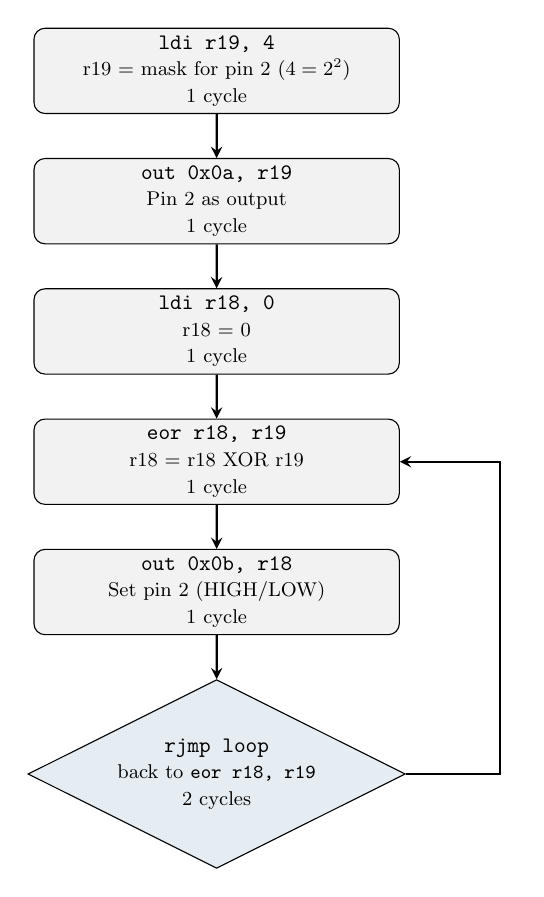
\begin{tikzpicture}[
    scale=0.8,
    every node/.style={transform shape},
    node distance=0.7cm and 0.8cm,
    box/.style={
        rectangle, draw,
        rounded corners,
        minimum width=5.8cm,
        minimum height=1.2cm,
        text centered,
        align=center,
        draw=black,
        fill=gray!10
    }
]

\node (step1) [box]
    {\texttt{ldi r19, 4} \\\small r19 = mask for pin 2 ($4 = 2^2$) \\\small 1 cycle};
\node (step2) [box, below=of step1]
    {\texttt{out 0x0a, r19} \\\small Pin 2 as output \\\small 1 cycle};
\node (step3) [box, below=of step2]
    {\texttt{ldi r18, 0} \\\small r18 = 0 \\\small 1 cycle};
\node (step4) [box, below=of step3]
    {\texttt{eor r18, r19} \\\small r18 = r18 XOR r19 \\\small 1 cycle};
\node (step5) [box, below=of step4]
    {\texttt{out 0x0b, r18} \\\small Set pin 2 (HIGH/LOW) \\\small 1 cycle};
\node (step6) [jump, below=of step5]
    {\texttt{rjmp loop} \\\small back to \texttt{eor r18, r19} \\\small 2 cycles};

\draw [arrow] (step1) -- (step2);
\draw [arrow] (step2) -- (step3);
\draw [arrow] (step3) -- (step4);
\draw [arrow] (step4) -- (step5);
\draw [arrow] (step5) -- (step6);

% jump back
\draw [arrow] (step6.east) -- ++(1.5,0) node[right] {}
              |- (step4.east);

\end{tikzpicture}
}
\end{center}


\newpage
\section{A simple delay with one register}

Our next goal is to make pin 2 switch between HIGH and LOW somewhat more
slowly. Ultimately, it should be possible to connect an LED there that then
blinks at a given frequency that is perceptible to the eye.

A little spoiler: with the current approach, the LED would blink at about
20,000 hertz – that would still not be perceptible to the eye (even if it
were technically possible to switch an LED on and off at such a high
frequency).

But the idea we develop and implement here can easily be improved to reach
our goal in the next section.
Compared to \autoref{lst:led_pin2_xor}, the code shown in
\autoref{lst:led_pin2_delay1} contains three additional instructions, which
have been added in lines 7 to 10:

\begin{itemize}
    \item
	The instruction in line~7 initializes register \texttt{r24} with the
	value~2. This register serves as a counter for a countdown and can of
	course also be loaded with other values. However, since registers on
	our microcontroller are only 8~bits wide, only values from \texttt{0}
	to \texttt{255} (or, in hexadecimal notation, from \texttt{0x00} to
	\texttt{0xFF}) are possible.

    \item
	The instruction in line~9 decrements register \texttt{r24} by~1.
	Technically, the value \texttt{1} is subtracted from \texttt{r24} and
	the result is stored back in \texttt{r24}. What matters here is that
	this subtraction computes not only the arithmetic result but also
	so-called \emph{status flags}. One of them is the so-called
	\emph{zero flag}, which is set exactly when the result of the
	subtraction equals~0.

    \item
	The instruction in line~10 is a conditional jump. \texttt{brne}
	stands for \enquote{Branch if Not Equal} and means: the jump to the
	label \texttt{delay} is taken only if the zero flag is \emph{not}
	set – that is, exactly when \texttt{r24} is not yet~0 after the last
	subtraction. If, on the other hand, the zero flag is set (i.e.,
	\texttt{r24} is now~0), execution continues with the next instruction
	in line~12.
\end{itemize}

\noindent
\autoref{fig:delay1} shows a flowchart for the program in
\autoref{lst:led_pin2_delay1}. It makes clear that the newly inserted lines
implement an inner loop in which register \texttt{r24} is counted down. This
loop is embedded in an outer loop that sets pin~2 alternately \texttt{HIGH}
and \texttt{LOW}.

The larger the initial value of \texttt{r24}, the more cycles are needed to
run through the inner loop before the state of pin~2 is changed again. The
time that pin~2 remains in a particular state (i.e., \texttt{HIGH} or
\texttt{LOW}) can thus be controlled deliberately.


\begin{listing}[htbp]
\begin{lstlisting}[
    frame=topbottom,
    numbers=left,
    numberstyle=\scriptsize,
    caption={
	\texttt{led\_pin2\_delay1.s} – pin 2 is toggled with a delay by means
	of a countdown loop in \texttt{r24}
    },
    captionpos=b,
    label={lst:led_pin2_delay1}
]
        ldi     r19,    4           ; 1 cycle
        out     0x0a,   r19         ; 1 cycle
        ldi     r18,    0           ; 1 cycle
loop:
        eor     r18,    r19         ; 1 cycle
        out     0x0b,   r18         ; 1 cycle
	ldi     r24,    0x2         ; 1 cycle (set countdown counter)
delay:
        subi    r24,    1           ; 1 cycle
        brne    delay               ; 2 cycles if jump taken, 1 cycle otherwise

        rjmp    loop                ; 2 cycles
\end{lstlisting}
\end{listing}

\begin{figure}[htbp]
\centering
\begin{center}
\scalebox{0.75}{%
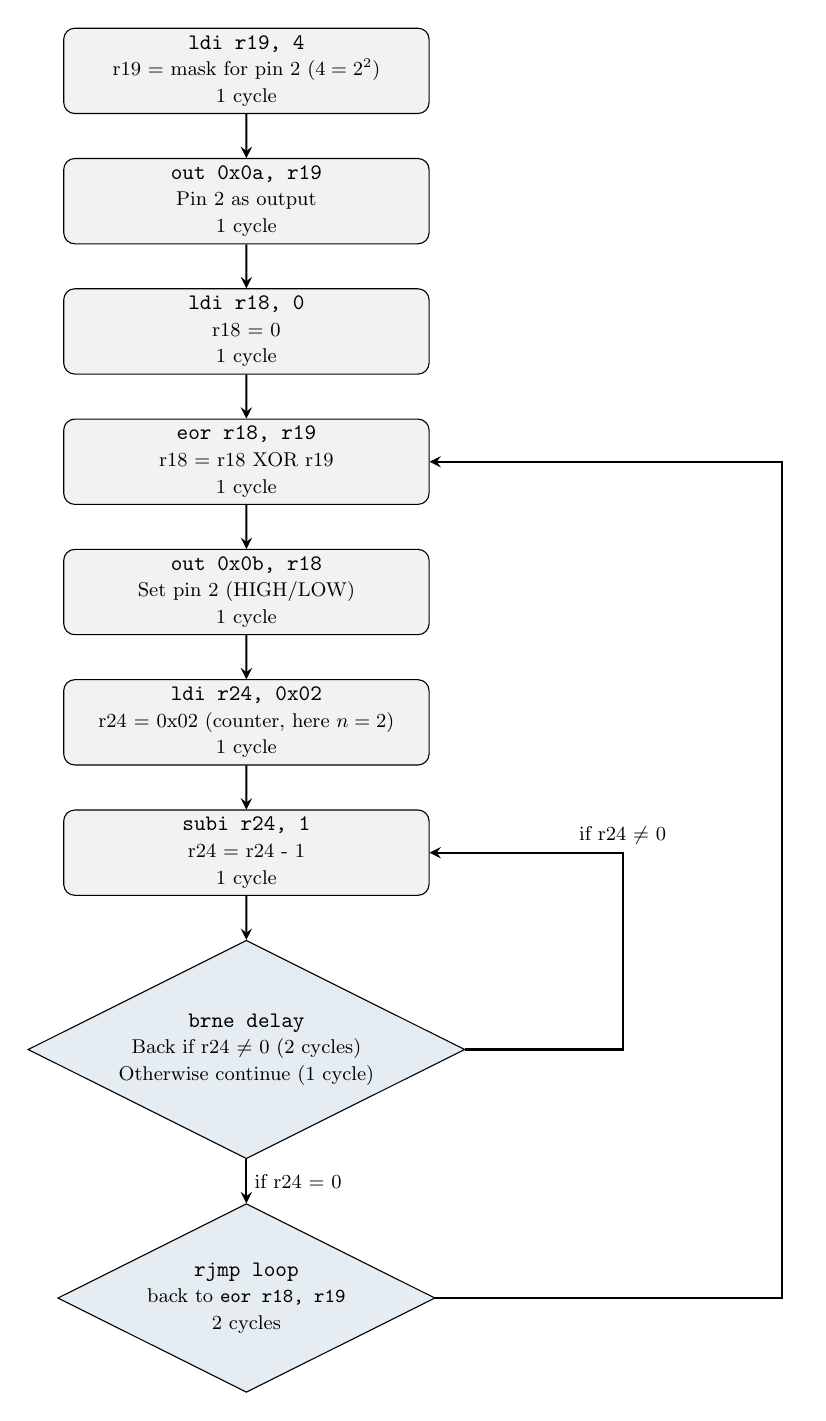
\begin{tikzpicture}[
    scale=0.8,
    every node/.style={transform shape},
    node distance=0.7cm and 0.8cm,
    box/.style={
        rectangle, draw,
        rounded corners,
        minimum width=5.8cm,
        minimum height=1.2cm,
        text centered,
        align=center,
        draw=black,
        fill=gray!10
    }
]
\node (step1) [box]
    {
	\texttt{ldi r19, 4} \\
	\small r19 = mask for pin 2 ($4 = 2^2$) \\
	\small 1 cycle
    };
\node (step2) [box, below=of step1]
    {
	\texttt{out 0x0a, r19} \\
	\small Pin 2 as output \\
	\small 1 cycle
    };
\node (step3) [box, below=of step2]
    {
	\texttt{ldi r18, 0} \\
	\small r18 = 0 \\
	\small 1 cycle
    };
\node (step4) [box, below=of step3]
    {
	\texttt{eor r18, r19} \\
	\small r18 = r18 XOR r19 \\
	\small 1 cycle
    };
\node (step5) [box, below=of step4]
    {
	\texttt{out 0x0b, r18} \\
	\small Set pin 2 (HIGH/LOW) \\
	\small 1 cycle
    };
\node (step6) [box, below=of step5]
    {
	\texttt{ldi r24, 0x02} \\
	\small r24 = 0x02 (counter, here $n=2$)\\
	\small 1 cycle
    };
\node (step7) [box, below=of step6]
    {
	\texttt{subi r24, 1} \\
	\small r24 = r24 - 1 \\
	\small 1 cycle
    };
\node (step8) [jump, below=of step7]
    {
	\texttt{brne    delay} \\
	\small Back if r24 $\neq$ 0 (2 cycles)\\
	\small Otherwise continue (1 cycle)
    };
\node (step9) [jump, below=of step8]
    {
	\texttt{rjmp loop} \\
	\small back to \texttt{eor r18, r19} \\
	\small 2 cycles
    };
\draw [arrow] (step1) -- (step2);
\draw [arrow] (step2) -- (step3);
\draw [arrow] (step3) -- (step4);
\draw [arrow] (step4) -- (step5);
\draw [arrow] (step5) -- (step6);
\draw [arrow] (step6) -- (step7);
\draw [arrow] (step7) -- (step8);
\draw [arrow] (step8) -- (step9) node[midway, right] {\small if r24 = 0};

% jump back
\draw [arrow] (step8.east) -- ++(2.5,0)
	      |- (step7.east) node[midway, above] {\small if r24 $\neq$ 0};
\draw [arrow] (step9.east) -- ++(5.5,0) node[right] {}
	      |- (step4.east);

\end{tikzpicture}
}
\end{center}
\caption{
    Flowchart for the program from \autoref{lst:led_pin2_delay1} with a
    delay loop using \texttt{r24}. The outer loop changes the pin state, the
    inner loop produces a variable pause.
}
\label{fig:delay1}
\end{figure}

\vspace{53bp}
\subsection{Clock cycles per loop iteration}

We now want to compute how many clock cycles elapse between two consecutive
executions of the \texttt{eor} instruction in line~5 – that is, how long it
takes until the state of pin~2 changes again.

The decisive factor is how often the inner loop is executed. If register
\texttt{r24} is initialized with a value \( n \), the loop is executed
\( n \) times in total. The jump back to the label \texttt{delay} is taken
exactly \( n-1 \) times. The \( n \)-th time, the result of the subtraction
is zero, the zero flag is set, and no jump is taken anymore.

\newpage

\noindent
According to the datasheet, the \texttt{subi} instruction (line~9) always
takes 1 cycle. The \texttt{brne} instruction (line~10) takes:
\begin{itemize}
  \item 2 cycles if the jump is taken (\( n-1 \) times),
  \item 1 cycle if no jump is taken (once).
\end{itemize}
The inner loop (lines~9–10) thus takes a total of:
\[
(n-1) \cdot (1 + 2) + 1 + 1 = 3(n-1) + 2 \quad \text{cycles}
\]
In addition, the following instructions are executed before and after this
loop:
\begin{itemize}
  \item Line~7: \texttt{ldi r24, n} → 1 cycle
  \item Line~6: \texttt{out 0x0b, r18} → 1 cycle
  \item Line~5: \texttt{eor r18, r19} → 1 cycle
  \item Line~12: \texttt{rjmp loop} → 2 cycles
\end{itemize}
This gives a total of:
\[
3(n-1) + 2 + 3 + 2 = 3n + 4 \quad \text{cycles per loop iteration.}
\]
So the larger the initial value \( n \), the longer it takes until the state
at pin~2 changes again.


\vspace{14bp}
\subsection{Measuring the delay}

The following table shows how many clock cycles are needed for one iteration
of the outer loop, depending on the initial value \( n \) in register
\texttt{r24}. According to the previous derivation, the number of cycles
is:
\begin{equation}
    \label{eq:delay1}
    T(n) = 3(n - 1) + 7 = 3n + 4
\end{equation}
On a microcontroller running at 16\,MHz, one clock cycle lasts exactly
\( \SI{62.5}{\nano\second} \).
For various values of \( n \), \autoref{tab:delaytimes} shows how many
cycles and how much time a complete iteration of the outer loop takes.
Of course, we will measure this in the lab. It is helpful to first check,
for small values of \( n \), how long pin 2 stays HIGH and LOW,
respectively, in order to validate the formula from \eqref{eq:delay1}.

\begin{table}[H]
\centering
\begin{tabular}{c c c c}
\toprule
Initial value \( n \) & Cycles & Time in \si{\micro\second} & Time in \si{\nano\second} \\
\midrule
1   & 7   & 0.4375  & 437.5 \\
2   & 10  & 0.6250  & 625 \\
3   & 13  & 0.8125  & 812.5 \\
4   & 16  & 1.0000  & 1000 \\
255 & 769 & 48.0625 & 48062.5 \\
\bottomrule
\end{tabular}
\caption{Delay per loop iteration for various initial values}
\label{tab:delaytimes}
\end{table}


\newpage
\section{A longer delay with four registers}

\begin{listing}[htbp]
\begin{lstlisting}[
    frame=topbottom,
    numbers=left,
    numberstyle=\scriptsize,
    caption={
	Program \texttt{led\_pin2\_delay4.s}: four registers
	(\texttt{r24} to \texttt{r27}) are used as a 32-bit counter to
	produce a much longer delay. Pin 2 is still toggled with each
	iteration of the outer loop.
    },
    captionpos=b,
    label={lst:led_pin2_delay4}
]
        ldi     r19,    4           ; for pin 2 (4 = 2^2)
        out     0x0a,   r19
        ldi     r18,    0
loop:
        eor     r18,    r19         ; 1 cycle
        out     0x0b,   r18         ; 1 cycle

        ldi     r24,    0x54        ; 1 cycle
        ldi     r25,    0x58        ; 1 cycle
        ldi     r26,    0x14        ; 1 cycle
        ldi     r27,    0x00        ; 1 cycle
delay:
        subi    r24,    1           ; 1 cycle
        sbci    r25,    0           ; 1 cycle
        sbci    r26,    0           ; 1 cycle
        sbci    r27,    0           ; 1 cycle
        brne    delay               ; 2 cycles if jump taken, 1 cycle otherwise

        rjmp    loop                ; 2 cycles
\end{lstlisting}
\end{listing}


\noindent
To achieve a longer delay, we need more than 8 bits for the countdown
counter. The program shown in \autoref{lst:led_pin2_delay4} therefore uses a
32-bit counter implemented with the four registers \texttt{r24} to
\texttt{r27}. These are treated as a register group and counted down
together to achieve a much longer delay than with just a single register.

A \emph{register group} means interpreting several consecutive 8-bit
registers as one common larger register, in our case a 32-bit counter. Each
register stores one byte of the total value, with \texttt{r24} holding the
least significant byte and \texttt{r27} the most significant byte. For
example, the following assignment

\begin{center}
    \texttt{r24 = 0x12}, \quad \texttt{r25 = 0x34},
    \quad \texttt{r26 = 0x56}, \quad \texttt{r27 = 0x78}
\end{center}

\noindent
corresponds to the combined value
\[
    n = \texttt{r27:r26:r25:r24} = \texttt{0x78563412}.
\]
In \autoref{lst:led_pin2_delay4}, the counter is initialized in lines 8 to 11
with four \texttt{ldi} instructions. There we get
\[
    n = \texttt{r27:r26:r25:r24} = \texttt{0x00000200} = 512,
\]
which means that the loop is executed 512 times before the state of pin 2 is
changed again.

\newpage
\noindent
Our microprocessor has no instruction for directly decrementing a register
group of four registers%
\footnote{For a register group of two registers,
e.g., \texttt{r25:r24}, there is the \texttt{SBIW} instruction
(Subtract Immediate from Word).}.
However, such an operation can be emulated by a combination of \texttt{subi}
(subtract immediate) and \texttt{sbci} (subtract immediate with carry).
This is done in lines~13 to~16
of \autoref{lst:led_pin2_delay4}:

\begin{lstlisting}[language={},numbers=none]
        subi    r24,    1
        sbci    r25,    0
        sbci    r26,    0
        sbci    r27,    0
\end{lstlisting}

\noindent
Put simply, these four instructions have the effect that the entire 32-bit
value in the register group \texttt{r27:r26:r25:r24} is decremented by one.
As soon as the value has reached zero (i.e., all four registers contain the
value \texttt{0x00}), the zero flag in the status register is set –
otherwise it remains cleared.

\vspace{1em}
\noindent
\textbf{In more detail:} The \texttt{subi} instruction subtracts the
value~1 from \texttt{r24} and in doing so sets the flags in the status
register, among them the carry flag (C) if a borrow occurred. Two typical
cases:
\begin{itemize}
    \item
	\textbf{Case 1:} \texttt{r24 = 0x01} before the subtraction.\\
	After \texttt{subi r24, 1}, \texttt{r24 = 0x00}, and no borrow
	occurs; the carry flag remains cleared.
    \item
	\textbf{Case 2:} \texttt{r24 = 0x00} before the subtraction.\\
	After \texttt{subi r24, 1}, \texttt{r24 = 0xFF}, since the
	subtraction underflows. In this case, the carry flag is set.
\end{itemize}
In general: with \texttt{subi}, the carry flag is set exactly when
\texttt{r24} had the value \texttt{0x00} before the subtraction, i.e., when a
borrow occurs when subtracting 1.

The subsequent \texttt{sbci} instructions then each subtract the value~0
\emph{taking into account} the carry flag. If, e.g., there was a borrow when
decrementing \texttt{r24} (because it was 0 before), this borrow is
propagated to \texttt{r25}, so that the group is correctly decremented by 1.
The chaining of these four instructions thus emulates a correct 32-bit
decrement.
The zero flag is set only if the result of the entire operation is zero,
i.e., all four registers contain \texttt{0x00} and there was no further
borrow after the last \texttt{sbci} instruction.

\subsection{Clock cycles per loop iteration}

\autoref{fig:delay4} shows a flowchart for \autoref{lst:led_pin2_delay4}.
Although we have considerably more instructions than with the one-register
delay, the structure is very similar: an inner loop for the delay and an
outer one for toggling pin 2.

So we can determine in the same way how many clock cycles elapse until the
state of pin 2 changes again.
If \( n \) is the value of the register group \texttt{r27:r26:r25:r24},
then the inner loop takes
\[
    (n - 1) \cdot 6 + 5
\]
cycles. The outer loop contains further instructions that together take
8 cycles. Altogether, this gives:
\[
    T(n) = (n - 1) \cdot 6 + 5 + 8 = 6n + 7
\]
\newpage
\noindent
This can be checked for a few example values:
\begin{itemize}
    \item
	\( n = 1 \Rightarrow T(1) = 13 \) cycles
	\( \Rightarrow 13 \cdot 62.5\,\text{ns} = 812.5\,\text{ns} \)
    \item
	\( n = 2 \Rightarrow T(2) = 19 \) cycles
	\( \Rightarrow 19 \cdot 62.5\,\text{ns} = 1187.5\,\text{ns} \)
\end{itemize}
An even more interesting question is which value of \( n \) you have to
choose so that pin 2 blinks at a frequency of 1\,Hz, i.e., is HIGH for
500\,ms and LOW for 500\,ms. For this, the following must hold:
\[
    (6n + 7) \cdot 62.5\,\text{ns}
	= 500\,\text{ms} = 500\,000\,000\,\text{ns}
\]
Solving this equation for \( n \) gives:
\[
    n = \frac{500\,000\,000 / 62.5 - 7}{6}
	= \frac{8\,000\,000 - 7}{6} = 1\,333\,332.166\ldots
\]
Since we can only use integer values for \( n \), we choose:
\[
n = 1\,333\,332 = \texttt{0x145854}
\]
This value is within our measurement accuracy and ensures that a connected
LED blinks at about 1\,Hz.


\begin{figure}[htbp]
\centering
\begin{center}
\scalebox{0.75}{%
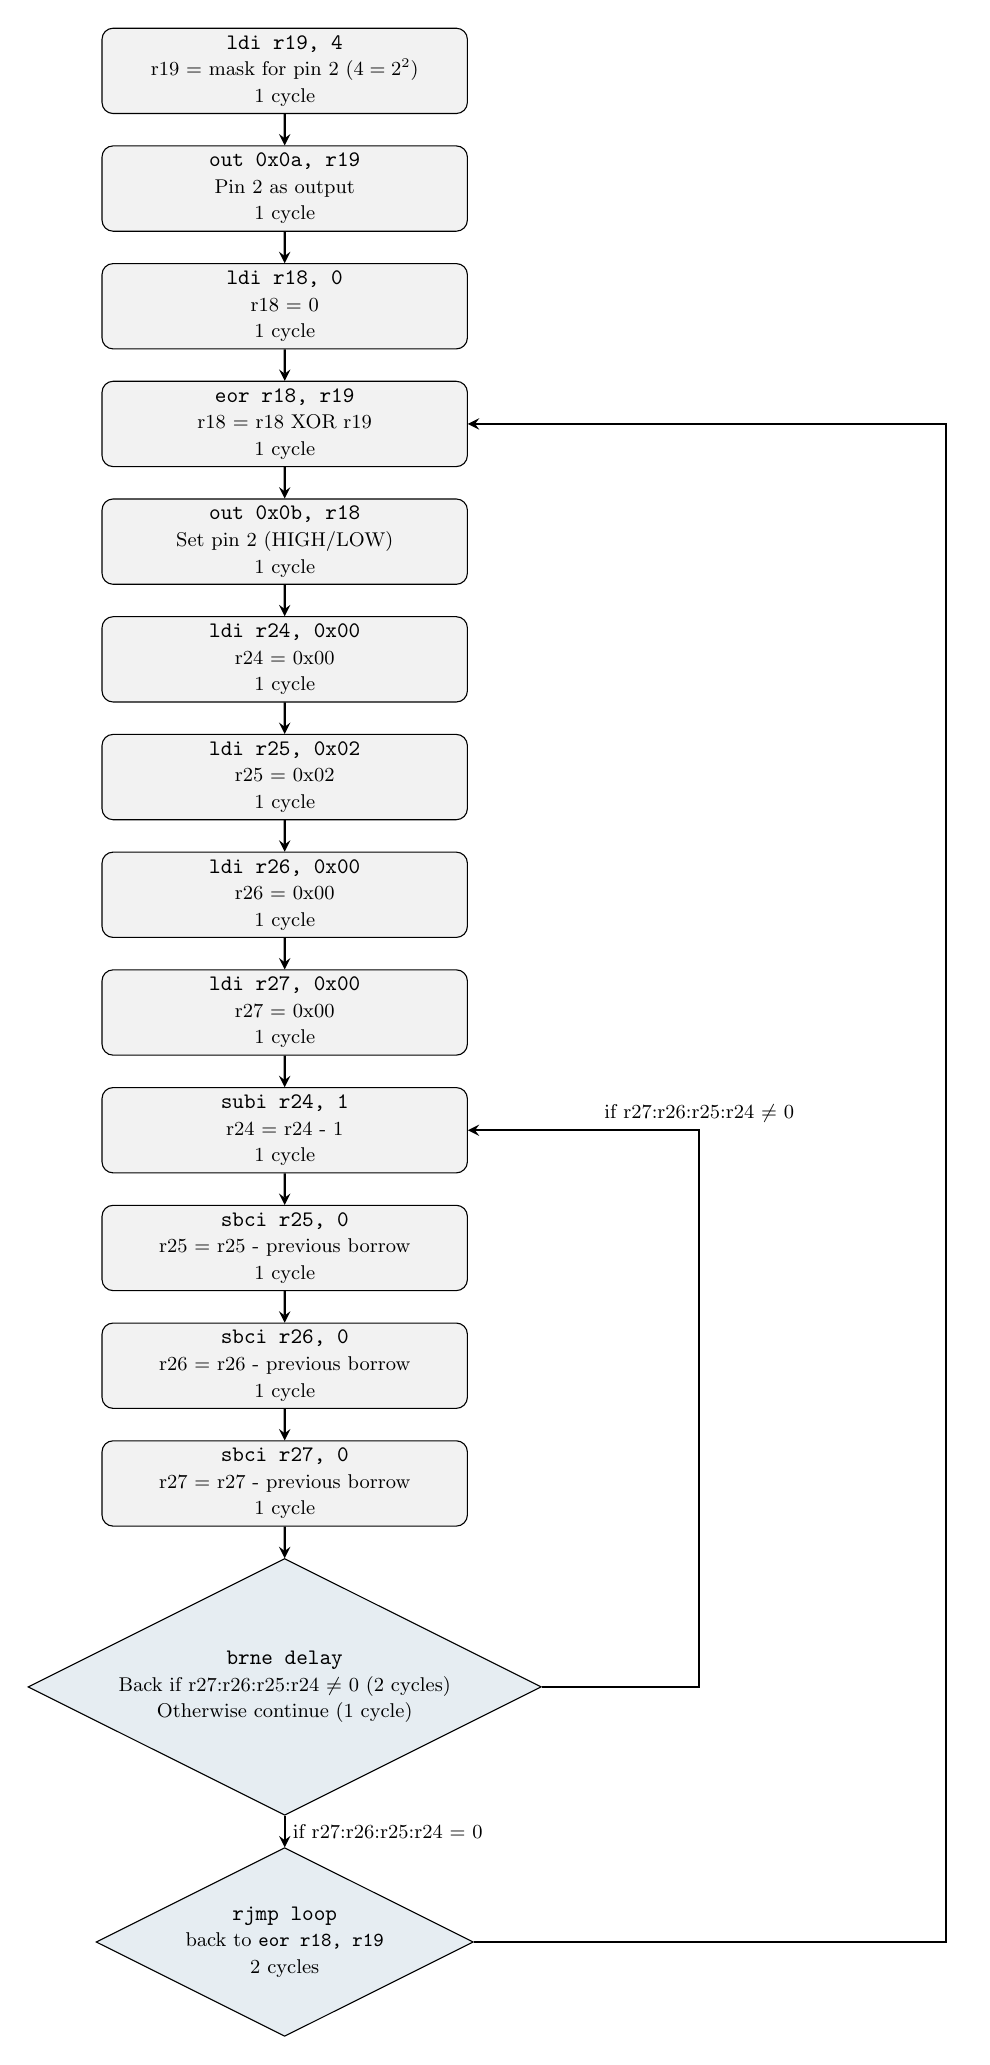
\begin{tikzpicture}[
    scale=0.8,
    every node/.style={transform shape},
    node distance=0.5cm and 0.7cm,
    box/.style={
        rectangle, draw,
        rounded corners,
        minimum width=5.8cm,
        minimum height=1.2cm,
        text centered,
        align=center,
        draw=black,
        fill=gray!10
    }
]
\node (step1) [box]
    {
	\texttt{ldi r19, 4} \\
	\small r19 = mask for pin 2 ($4 = 2^2$) \\
	\small 1 cycle
    };
\node (step2) [box, below=of step1]
    {
	\texttt{out 0x0a, r19} \\
	\small Pin 2 as output \\
	\small 1 cycle
    };
\node (step3) [box, below=of step2]
    {
	\texttt{ldi r18, 0} \\
	\small r18 = 0 \\
	\small 1 cycle
    };
\node (step4) [box, below=of step3]
    {
	\texttt{eor r18, r19} \\
	\small r18 = r18 XOR r19 \\
	\small 1 cycle
    };
\node (step5) [box, below=of step4]
    {
	\texttt{out 0x0b, r18} \\
	\small Set pin 2 (HIGH/LOW) \\
	\small 1 cycle
    };
\node (step6) [box, below=of step5]
    {
	\texttt{ldi r24, 0x00} \\
	\small r24 = 0x00\\
	\small 1 cycle
    };
\node (step7) [box, below=of step6]
    {
	\texttt{ldi r25, 0x02} \\
	\small r25 = 0x02\\
	\small 1 cycle
    };
\node (step8) [box, below=of step7]
    {
	\texttt{ldi r26, 0x00} \\
	\small r26 = 0x00\\
	\small 1 cycle
    };
\node (step9) [box, below=of step8]
    {
	\texttt{ldi r27, 0x00} \\
	\small r27 = 0x00\\
	\small 1 cycle
    };
\node (step10) [box, below=of step9]
    {
	\texttt{subi r24, 1} \\
	\small r24 = r24 - 1 \\
	\small 1 cycle
    };
\node (step11) [box, below=of step10]
    {
	\texttt{sbci r25, 0} \\
	\small r25 = r25 - previous borrow  \\
	\small 1 cycle
    };
\node (step12) [box, below=of step11]
    {
	\texttt{sbci r26, 0} \\
	\small r26 = r26 - previous borrow  \\
	\small 1 cycle
    };
\node (step13) [box, below=of step12]
    {
	\texttt{sbci r27, 0} \\
	\small r27 = r27 - previous borrow  \\
	\small 1 cycle
    };
\node (step14) [jump, below=of step13]
    {
	\texttt{brne    delay} \\
	\small Back if r27:r26:r25:r24 $\neq$ 0 (2 cycles)\\
	\small Otherwise continue (1 cycle)
    };
\node (step15) [jump, below=of step14]
    {
	\texttt{rjmp loop} \\
	\small back to \texttt{eor r18, r19} \\
	\small 2 cycles
    };
\draw [arrow] (step1) -- (step2);
\draw [arrow] (step2) -- (step3);
\draw [arrow] (step3) -- (step4);
\draw [arrow] (step4) -- (step5);
\draw [arrow] (step5) -- (step6);
\draw [arrow] (step6) -- (step7);
\draw [arrow] (step7) -- (step8);
\draw [arrow] (step8) -- (step9);
\draw [arrow] (step9) -- (step10);
\draw [arrow] (step10) -- (step11);
\draw [arrow] (step11) -- (step12);
\draw [arrow] (step12) -- (step13);
\draw [arrow] (step13) -- (step14);
\draw [arrow] (step14) -- (step15) node[midway, right]
    {\small if r27:r26:r25:r24 = 0};

% jump back
\draw [arrow] (step14.east) -- ++(2.5,0)
	      |- (step10.east) node[midway, above]
		{\small if r27:r26:r25:r24 $\neq$ 0};
\draw [arrow] (step15.east) -- ++(7.5,0) node[right] {}
	      |- (step4.east);

\end{tikzpicture}
}
\end{center}
\caption{
    Flowchart for the program \texttt{led\_pin2\_delay4.s}. The countdown
    uses a 32-bit register group (\texttt{r27:r26:r25:r24}). The diagram
    shows how the inner loop with \texttt{subi}/\texttt{sbci}/\texttt{brne}
    produces a longer delay before the state of pin 2 is changed again in
    the outer loop.
}
\label{fig:delay4}
\end{figure}


\newpage
\section{Bare-metal C}

\begin{listing}[htbp]
\begin{lstlisting}[
    frame=topbottom,
    numbers=left,
    numberstyle=\scriptsize,
    caption={
	C program \texttt{led\_pin2\_delay.c}, which produces almost the same
	assembly code as the handwritten version in
	\autoref{lst:led_pin2_delay4}.
	The LED at pin 2 is toggled with exactly the same delay. Differences
	in the generated assembly code (\autoref{lst:led_pin2_delay_s}) are
	minimal and concern only irrelevant details.
    },
    captionpos=b,
    label={lst:led_pin2_delay_c}
]
static void setPinModes(unsigned char mode)
{
    *(volatile unsigned char *)(0x2A) = mode;
}

static void digitalWriteAll(unsigned char val)
{
    *(volatile unsigned char *)(0x2B) = val;
}

static void delay_cycles(unsigned long count)
{
    do {
        // compiler should use registers for count
        asm volatile ("" : "+r"(count));
        count = count - 1;
    } while (count != 0);
}

int main()
{
    // setup
    unsigned char pin = 2;
    unsigned char pinModes = 1 << pin;
    setPinModes(pinModes);

    unsigned char pinValues = 0;
    while (1) {
        // loop
        pinValues ^= 1 << pin;
        digitalWriteAll(pinValues);
        delay_cycles((500000000 / 62.5 - 7) / 6);
    }
}
\end{lstlisting}
\end{listing}

\noindent
What actually happens when you click ``Upload'' in the Arduino IDE? With the
knowledge from this project, we can now answer this question – and carry out
the individual steps ourselves. In this last section, we move up from machine
code to C, but stay very close to the hardware: no libraries, no magic – bare
metal.

\subsection{A C program for a blinking LED}
\autoref{lst:led_pin2_delay_c} shows a C program that makes an LED connected
to pin 2 blink at a frequency of 1\,Hz. If you look at the code, you may see
that there is some magic involved after all.
The code in lines 1 to 18 is not for the faint of heart and requires not only
a somewhat deeper understanding of the C programming language and of how a C
compiler generates machine code from it, but also knowledge of the
microprocessor. Here, for example, the addresses \texttt{0x2A} and
\texttt{0x2B} are used to configure pin 2 as an output and to set it HIGH or
LOW, respectively.

But here is the point: an end user does not need to understand how the code
in lines 1 to 18 works in order to use it. Because ultimately, all it does is
provide easy-to-use functions:
\begin{itemize}
  \item
      \texttt{setPinModes} – to configure pins as inputs or outputs,
  \item
      \texttt{digitalWriteAll} – to set pins HIGH or LOW,
  \item
      \texttt{delay\_cycles} – to wait for a certain number of clock cycles.
\end{itemize}

\noindent
The implementation of these functions can be hidden in a library; you then
only need to know what these functions do and how to use them. For Arduino,
there is very good documentation for this.

As a user, you then only have to write the code in lines 20 to 34 yourself.
And even this part can be simplified further.

So the point here is \textbf{not} to understand this particular C code in
detail – after all, we will use the Arduino development environment later,
and with it things are much easier.
The aim here is merely to show that, in principle, a few lines of C code can
implement exactly what we programmed in assembly language before:
a blinking LED, directly on the hardware, without libraries, very close to
the metal.



\vspace{29bp}
\subsection{Toolchain}
\begin{figure}[ht]
\centering
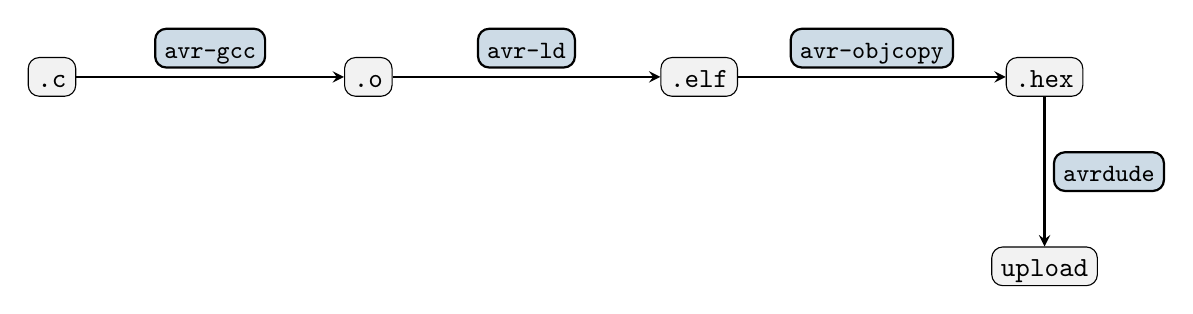
\begin{tikzpicture}[
  node distance=1.4cm and 3.4cm,
  every node/.style={draw, rounded corners, fill=gray!10, font=\ttfamily},
  arrow/.style={->, thick, >=stealth},
  text height=1.7ex,
  text depth=0pt,
  minimum height=1.8ex,
  align=center
]

\node (s)   {.c};
\node (o)   [right=of s] {.o};
\node (elf) [right=of o] {.elf};
\node (hex) [right=of elf] {.hex};
\node (upload) [below=of hex, yshift=-0.5cm] {upload};

\draw[arrow] (s)   -- (o)     node[midway, above=3pt, fill=myblue!20]  {\small avr-gcc};
\draw[arrow] (o)   -- (elf)   node[midway, above=3pt, fill=myblue!20]  {\small avr-ld};
\draw[arrow] (elf) -- (hex)   node[midway, above=3pt, fill=myblue!20]  {\small avr-objcopy};
\draw[arrow] (hex) -- (upload) node[midway, right=3pt, fill=myblue!20] {\small avrdude};

\end{tikzpicture}
\caption{
    Dependency graph for generating a \texttt{.hex} file and the subsequent
    upload. The tools \texttt{avr-gcc}, \texttt{avr-ld}, and
    \texttt{avr-objcopy} generate the \texttt{.hex} file, which is finally
    transferred to the microcontroller by \texttt{avrdude}.
}
\label{fig:makegraph_c}
\end{figure}

\noindent
The toolchain has now changed slightly: the C compiler can generate machine
code directly from the C code in the form of an object file. This
\texttt{.o} file is then processed, as before, by the linker and other tools
until a \texttt{.hex} file is produced at the end. An overview of this process
is shown in \autoref{fig:makegraph_c}. Of course, you can use a Makefile as
in \autoref{lst:Makefile_c} so that you do not have to type every command
every time. And with that, the secret is actually already revealed:

\begin{tcolorbox}[
	colback=myblue!5!white, colframe=myblue,
	title=What happens when you click ``Upload''?
]
If you type in a program like the one in \autoref{lst:led_pin2_delay_c} and
press the Upload button, a command like

\texttt{make upload HEX=led\_pin2\_delay.hex}

is executed internally, which automatically runs through the complete
toolchain.
\end{tcolorbox}

\noindent
We can also enter this command manually on the command line and observe what
happens:

\begin{lstlisting}
MCL:c lehn$ make upload HEX=led_pin2_delay.hex
avr-gcc -mmcu=atmega328p -c -Os -o led_pin2_delay.o led_pin2_delay.c
avr-ld -mavr5 -o led_pin2_delay.elf led_pin2_delay.o
avr-objcopy -O ihex -R .eeprom led_pin2_delay.elf led_pin2_delay.hex
avrdude -c arduino -P /dev/cu.usbserial-01C5FB3D -p atmega328p -U flash:w:led_pin2_delay.hex:i
Reading 30 bytes for flash from input file led_pin2_delay.hex
Writing 30 bytes to flash
Writing | ################################################## | 100% 0.03 s
Reading | ################################################## | 100% 0.01 s
30 bytes of flash verified

Avrdude done.  Thank you.
rm led_pin2_delay.elf led_pin2_delay.o
\end{lstlisting}

\begin{listing}[htbp]
\begin{lstlisting}[
    frame=topbottom,
    numbers=left,
    numberstyle=\scriptsize,
    caption={
	\texttt{Makefile} for translating C and assembly programs on Linux and
	macOS. This version processes both \texttt{.c} files and \texttt{.s}
	files and automatically generates matching \texttt{.hex} files. An
	optional target \texttt{upload} detects the serial interface
	automatically and transfers the program via \texttt{avrdude}.
    },
    captionpos=b,
    label={lst:Makefile_c}
]
# This version processes assembly programs (*.s)
# and C programs (*.c)

ASM_SOURCES := $(wildcard *.s)
C_SOURCES := $(wildcard *.c)
OBJECTS := $(ASM_SOURCES:.s=.o) $(C_SOURCES:.c=.o)
ELFS    := $(OBJECTS:.o=.elf)
HEXS    := $(ELFS:.elf=.hex)

all: $(HEXS)

%.o: %.c
        avr-gcc -mmcu=atmega328p -c -Os -o $@ $<

%.s: %.c
        avr-gcc -mmcu=atmega328p -S -Os -o $@ $<

%.o: %.s
        avr-as -o $@ $<

%.elf: %.o
        avr-ld -mavr5 -o $@ $<

%.hex: %.elf
        avr-objcopy -O ihex -R .eeprom $< $@

clean:
        $(RM) $(OBJECTS) $(ELFS) $(HEXS)

ifeq ($(MAKECMDGOALS),upload)
ifeq ($(shell uname), Linux)
PORT := $(shell ls /dev/ttyUSB* 2>/dev/null | head -n 1)
else
PORT := $(shell ls /dev/cu.usb* 2>/dev/null | head -n 1)
endif # uname
endif # MAKECMDGOALS == upload

upload: $(HEX)
        @if [ -z "$(HEX)" ]; then \
            echo "Usage: make upload HEX=<filename.hex>"; \
            false; \
        fi
        @if [ -z "$(PORT)" ]; then \
            echo "no USB device found"; \
            false; \
        fi
        avrdude -c arduino -P $(PORT) -p atmega328p -U flash:w:$(HEX):i
\end{lstlisting}
\end{listing}

\subsection{Generating readable assembly instead of machine code}

In the past, C compilers generated only assembly code, which was then
translated into machine code by an assembler. Today's compilers usually skip
this step and generate machine code directly, since an assembler is
practically already integrated into the compiler.

If you like, however, you can still have the generated assembly code output
– and that is exactly what is interesting in our case. Our Makefile helps us
call the compiler with the options required for this.
With the command

\begin{lstlisting}
MCL:c lehn$ make led_pin2_delay.s
avr-gcc -mmcu=atmega328p -S -Os -o led_pin2_delay.s led_pin2_delay.c
\end{lstlisting}

\noindent
the C code \texttt{led\_pin2\_delay.c} is translated into assembly code
(\texttt{led\_pin2\_delay.s}).

\autoref{lst:led_pin2_delay_s} shows the assembly code generated by the C
compiler \texttt{avr-gcc}. Only lines 16 to 32 are relevant here.
In fact, you could delete all the other lines and generate a \texttt{.hex}
file from the remaining lines that would not differ in functionality.

\newpage
\subsection{Comparison with our assembly program}

\begin{listing}[htbp]
\begin{lstlisting}[
    frame=topbottom,
    numbers=left,
    numberstyle=\scriptsize,
    caption={
	Assembly code \texttt{led\_pin2\_delay.s}, generated automatically by
	\texttt{avr-gcc} from the C program in \autoref{lst:led_pin2_delay_c}.
	The code differs from the handwritten version in
	\autoref{lst:led_pin2_delay4} in only two irrelevant details;
	in particular, the timing remains completely identical.
    },
    captionpos=b,
    label={lst:led_pin2_delay_s}
]
        .file   "led_pin2.c"
__SP_H__ = 0x3e
__SP_L__ = 0x3d
__SREG__ = 0x3f
__tmp_reg__ = 0
__zero_reg__ = 1
        .text
        .section        .text.startup,"ax",@progbits
.global main
        .type   main, @function
main:
/* prologue: function */
/* frame size = 0 */
/* stack size = 0 */
.L__stack_usage = 0
        ldi r18,lo8(4)
        out 0xa,r18
        ldi r18,0
        ldi r19,lo8(4)
.L3:
        eor r18,r19
        out 0xb,r18
        ldi r24,lo8(84)
        ldi r25,lo8(88)
        ldi r26,lo8(20)
        ldi r27,0
.L2:
        sbiw r24, 1
        sbci r26, 0
        sbci r27, 0
        brne .L2
        rjmp .L3
        .size   main, .-main
        .ident  "GCC: (Homebrew AVR GCC 14.2.0) 14.2.0"
\end{lstlisting}
\end{listing}

\noindent
Let us go through the differences from our handwritten assembly program step
by step:

\begin{enumerate}
\item
Lines 16 to 19 read:
\begin{lstlisting}[language={[x86masm]Assembler}]
ldi r18,lo8(4)
out 0xa,r18
ldi r18,0
ldi r19,lo8(4)
\end{lstlisting}

\newpage
\noindent
This is equivalent to:
\begin{lstlisting}[language={[x86masm]Assembler}]
ldi r18,4
out 0xa,r18
ldi r18,0
ldi r19,4
\end{lstlisting}
So the compiler has generated an unnecessary instruction here. Cleverer (and
shorter) would be:
\begin{lstlisting}[language={[x86masm]Assembler}]
ldi r19,4
out 0xa,r19
ldi r18,0
\end{lstlisting}
And that is exactly what we did in our program.

\item
Lines 20 to 22 read:
\begin{lstlisting}[language={[x86masm]Assembler}]
.L3:
eor r18,r19
out 0xb,r18
\end{lstlisting}
Our label is called \texttt{loop}, the compiler's is called \texttt{.L3}. The
rest is identical. What you call a label does not matter – humans prefer
meaningful names, compilers often use \texttt{.L} followed by a consecutive
number.

\item
Lines 23 to 26 read:
\begin{lstlisting}[language={[x86masm]Assembler}]
ldi r24,lo8(84)
ldi r25,lo8(88)
ldi r26,lo8(20)
ldi r27,0
\end{lstlisting}
This is equivalent to:
\begin{lstlisting}[language={[x86masm]Assembler}]
ldi r24, 84
ldi r25, 88
ldi r26, 20
ldi r27, 0
\end{lstlisting}
Writing the values in hexadecimal, as we do, gives:
\begin{lstlisting}[language={[x86masm]Assembler}]
ldi r24, 0x54
ldi r25, 0x58
ldi r26, 0x14
ldi r27, 0x00
\end{lstlisting}

\item
Lines 27 to 32 read:
\begin{lstlisting}[language={[x86masm]Assembler}]
.L2:
sbiw r24, 1
sbci r26, 0
sbci r27, 0
brne .L2
rjmp .L3
\end{lstlisting}
\newpage
\noindent
Our label is called \texttt{delay} instead of \texttt{.L2}, since we are
humans. Another difference is the first instruction:
\begin{lstlisting}[language={[x86masm]Assembler}]
sbiw r24, 1
\end{lstlisting}

\noindent
It takes 2 cycles and decrements the register pair \texttt{r25:r24}.
So it has the same effect as:
\begin{lstlisting}[language={[x86masm]Assembler}]
subi r24, 1
sbci r25, 0
\end{lstlisting}
The compiler uses \texttt{sbiw} here because this instruction – although it
takes exactly as many cycles as our variant with \texttt{subi} and
\texttt{sbci} – reduces the code size. \texttt{sbiw} occupies only 2 bytes
in flash, whereas two separate instructions would require 4 bytes in total.
Especially on microcontrollers with limited program memory, this is an
important advantage.
\end{enumerate}


\section{More fun with the C code}

We have seen that the C code is functionally equivalent to our assembly code.
Now, of course, you can also experiment with the C code.
For example, \autoref{lst:led_pin2_delay_c} contains the line:

\begin{lstlisting}
delay_cycles((500000000 / 62.5 - 7) / 6);
\end{lstlisting}

This has the effect that pin 2 is alternately HIGH for 500\,ms and then LOW
for 500\,ms. The number \texttt{n = 500000000} specifies the desired delay
in nanoseconds.

Of course, you can choose other values here as well – including very small
ones such as \texttt{n = 1} or \texttt{n = 2} – and use the oscilloscope to
verify that the behavior changes in exactly the same way as in our assembly
program.




\end{document}
